\documentclass[11pt]{book}

\usepackage[utf8]{inputenc}

\usepackage{etex}

\usepackage{url}

\usepackage{amscd}
\usepackage{amsmath, amstext, amsthm}
\usepackage{array}

\usepackage{hyperref}

\usepackage{enumerate}
\usepackage{pictex, color}
\usepackage{graphicx}

\usepackage{listings}
\usepackage{mathlist}

\usepackage{natbib}

\usepackage{tabularx}

\def\mail{\url{bastin@iro.umontreal.ca}}
\def\name{{\sf ORATIO}}
\def\version{0.7.4}

\def\MSE{\mbox{MSE}}
\def\RE{\mbox{RE}}
\def\Var{\mbox{Var}}

\def\blas{\texttt{BLAS}}
\def\cblas{\texttt{CBLAS}}
\def\lapack{\texttt{LAPACK}}

\def\openblas{\texttt{OpenBlas}}
\def\blasweb{\url{https://github.com/xianyi/OpenBLAS}}

\def\oratio{\name}

\newtheorem{thm}{Theorem}

\def\inullsep{\setlength{\itemsep}{0pt}}

\usepackage{makeidx}
\newcommand{\Index}[1]{#1\index{#1}}
\makeindex

\usepackage{mycal}
\usepackage{mybold}
\def\rit{\mathcal{R}}

\setcounter{secnumdepth}{5}

\begin{document}

\begin{titlepage}
{\Huge {\bf ORATIO Library}} 

{\huge Reference manual}

\vspace*{\stretch{1}}

%\includegraphics{delacroix.eps}
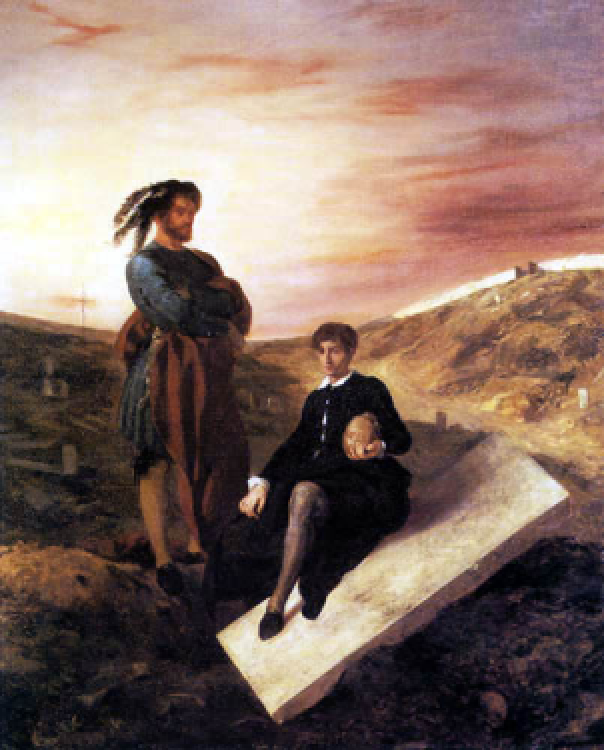
\includegraphics{delacroix.pdf}

\vspace*{\stretch{1}}

Fabian Bastin\hspace*{\stretch{1}}{\large  \today}

\date{}

\end{titlepage}

\tableofcontents

\chapter{Introduction}

\begin{quote}
\begin{flushright}
{\sl Heere sweet Lord, at your service.}\\
Horatio, The Tragedie of Hamlet.
\end{flushright}
\end{quote}

This document covers the version \version{} of the library \name{},
and is itself on a beta development level.
Any suggestion should be sent to \mail.

The library design is also subject to modifications, so please refer
to this documentation if you face linkage problems after the upgrade
of the library.
You can also consult the file \verb|ChangeLog| at the root of the
package, as well as in each subdirectories to read more specific
changes.

\section{A brief overview}

\name{} is a collection of sublibraries, each of then aiming to cover
some specific needs.
These components are
\begin{description}
\item[C Tools]: collection of basic C utilities;
\item[Data strucutres]: basic data structures as lists and trees;
\item[Numerical utilities]: various basic numerical tools, as finite
  and central difference, special functions,\ldots;
\item[Statistical tools]: basic statistical analysis and distributions
  properties routines;
\item[Random numbers]: (pseudo-)random numbers generation;
\item[Quasi-Monte Carlo]: quasi-Monte Carlo sequences generation.
\end{description}
Each of these parts is described in more details in the next chapters.
A set of example files is also provided in the directory \texttt{examples}.

\section{Requirements and installation}
\label{sec:requirements}

\subsection{Environment variables}

In order to allow the various libraries to be found during the
compilation process and execution, please add
the following lines in the file $\verb|.bashrc|$, present at the
root of your home directory:
\begin{verbatim}
export LIBRARY_PATH=/usr/local/lib:$LIBRARY_PATH
export LD_LIBRARY_PATH=/usr/local/lib:$LD_LIBRARY_PATH
\end{verbatim}
This line can be placed at any position position in the
\verb|.bashrc| file, but be careful to use a raw text editor. From a
text console, your can reach your home directory by simply enter the
command
\begin{verbatim}
cd
\end{verbatim}

The place where the program and the libraries will be installed may vary
following the operating system.
If you benefit from administration rights, the installation paths will
be typically \verb|/usr/local/bin| for the programs and
\verb|/usr/local/lib| for the libraries.
If you have not these rights, the typical locations will be
\verb|$HOME/bin| and \verb|$HOME/lib|, where \verb|$HOME| is the user
repertory.
%For reference, we will design by \verb|INSTALL_PATH| the path where the programs are installed.

\subsection{OpenBLAS}
\label{sec:blas}

\oratio{} makes heavy use of \cblas{}, the C version of \blas{} (Basic Linear Algebra Subroutines) functions, that have to be installed first.
Any library implementing these routines should be compatible, but could possibly
require the modification of the file \verb|configure.in| to be
detected.
A recommended version is \textsf{OpenBLAS}, available at \url{http://www.openblas.net}.
It is based on \textsf{GotoBLAS2}, available at \url{http://www.tacc.utexas.edu/research-development/tacc-software/gotoblas2}, a \blas{} implementation proposed by the University of Texas at Austin.
Praised as one of the best implementations, it has been released under BSD license in 2010, but is no more maintained.

\textsf{OpenBLAS} installation requires to compile its source code. At the time of writing, the last version was 0.2.14. First, extract the code and compile it with the commands
\begin{verbatim}
tar zxvf OpenBLAS-0.2.14.tar.gz
cd OpenBLAS-0.2.14
make
\end{verbatim}
If you do not have the utility \textsf{wget} installed, you will also have to manually downoad LAPACK on Netlib.
The considered version of OpenBLAS requires LAPACK 3.5.0, available at the address \url{http://www.netlib.org/lapack/#_lapack_version_3_5_0}, but newer versions of OpenBLAS could rely on more recent LAPACK distributions.
The LAPACK archive has to be copied in the OpenBLAS main directory.

After the compilation, you can install the library with the command
\begin{verbatim}
sudo make install
\end{verbatim}
assuming that your account has enough administration rights.
By default, OpenBLAS is installed in the directory \verb|/opt/OpenBLAS|, but it is possible to specify the installation directory using the option \verb|PREFIX|, for instance
\begin{verbatim}
sudo make PREFIX=/usr/local install
\end{verbatim}
Since \verb|/usr/local| is the directory where \oratio{} is installed by defaults, it is a good idea to centralize the installation inside this directory.

\subsection{\oratio{} installation}

Once these dependencies are satisfied, the library can
be installed with the following instructions:
\begin{verbatim}
./configure
make
sudo make install
\end{verbatim}
Optimization compilation options can be specified as arguments of \verb|configure|, for instance:
\begin{verbatim}
./configure CFLAGS=''-O2'' FFLAGS="-O2"
\end{verbatim}

This documentation can also be generated using the command
\begin{verbatim}
make pdf
\end{verbatim}
which however requires a proper installation of \LaTeX.

\section{Conventions}

$x(i)$ designs the $i$-th component of the vector $x$.
When comparing two vectors $x$ and $y$ in $\rit^n$, an inequality $x \leq y$ is meant componentwise,
that is $x(i) \leq y(i),\ i = 1,\ldots,n$.

\section{Credits}

The development of the library has been initiated at FUNDP - the University of
Namur (Belgium), continued at the CERFACS (Toulouse, France), and is
currently pursued at the Universit\'e de Montr\'eal (QC, Canada).

Various people have contributed to this library.
Their names is written at the beginning of concerned files, and the
complete list is reproduced here, by alphabetical order: Adrien
Bonneu, Cinzia Cirillo, Pierre Derian, Jordan Goblet, Gabriel Schwanen.

\section{Miscellaneous}

\name{} stands for {\sl Operational Research, A Toolbox in Operation}.
Most of the routines were partially or totally written during
the development of the software {\sf AMLET} ({\sl Another Mixed Logit
Estimation Tool}).
The name is a reference to the Shapekespeare's masterpiece Hamlet.
Horatio was the best friend of Hamlet, as the library \name{} is the
primary companion of the software {\sf AMLET}.

The painting of the front cover is due to Eug\`ene Delacroix, in 1835,
under the name {\sl  Hamlet and Horatio in the Graveyard}.



\chapter{C Tools}

While standard C libraries are quite comprehensive, it remains useful
to define some additional utilities in order to alleviate the
programming work, and sometimes improve the code portability.
The following set of routines and constants aims to achieve this goal.

\section{Constants}

Various constants are proposed, in order to improve code readibility.
First, two constants are defined to express boolean conditions:
\begin{itemize}
\item
{\sf TRUE}, defined as 1;
\item
{\sf FALSE}, defined as 0.
\end{itemize}
Note that the constants names are written in uppercase.
The number of bits associated to the various basic C types can also be
designed with the following constants:
\begin{verbatim}
CHARBITS
SHORTBITS
INTBITS
LONGBITS
PTRBITS
DOUBLEBITS
FLOATBITS
\end{verbatim}
The number of bits used for any other type can be computed with the
macro
\begin{verbatim}
CTOOLS_BITS(type)
\end{verbatim}

\begin{verbatim}
typedef void (*C_GENERIC)(void);
\end{verbatim}

\section{File gestion}

While C standard libraries have functions to read text and binary files, they
not always easy to use.
We encapsulate some functions to simplify some basic operations on text files.

\subsection{Reading}

It it possible to read all the content of a text file in one shot, with the
function
\begin{verbatim}
char *c_file_get_text(char *name, long *length)
\end{verbatim}
The content is copy, verbatim, into a newly memory allocated characters array,
and the special character EOF (for end-of-file) is added.
The variable pointed by length, if length is not NULL, contains the size of this
character array (include the EOF character).

The current line of the file can be obtained with the function
\begin{verbatim}
char *c_file_get_line(FILE *input);
\end{verbatim}
The returned string is newly allocated, so it has to be freed by the user.

\subsection{\Index{CSV} format}

A specific file format is the comma-separated
values\index{comma-separated values|see{CSV}} format, which is useful
to represent simple data.

If separator is set to \verb|\0|, the constant
\verb|C_CSV_DEFAULT_SEPARATOR| is used.
\begin{verbatim}
C_CSV *c_csv_new(char *separator)
\end{verbatim}
\begin{verbatim}
void c_csv_free(C_CSV *csv)
\end{verbatim}

\section{Memory management}

\begin{verbatim}
#define _malloc(type) ((type *)c_malloc(sizeof(type)))
#define _mallocs(nb, type) ((type *)c_malloc((nb)*sizeof(type)))
#define _realloc(ptr, type) ((type *)c_realloc(ptr, sizeof(type)))
#define _reallocs(ptr, nb, type) ((type *)c_realloc(ptr, (nb)*sizeof(type)))
#define _free(var) (if (var) free(var));
\end{verbatim}

\section{Timer}

The following functions aim to mesure the elapsed time when executing the program. The timer mesure the CPU time on Unix systems, but due to API differences, the record will be less reliable on Windows systems.
%  /**
%   * Initialize the internal timer.
%   */
\begin{verbatim}
void ctools_timer_init()
\end{verbatim}

%  /**
%   * Return the time used (in seconds) since the timer initialization.
%   *
%   * @param output is a pointer to the file where the time has to recorded,
%   *    or NULL if it does not to be recorded.
%   * @param sec contains on output the number of seconds.
%   * @param ms  contains on output the number of millseconds.
%   *
%   * @return the elapsed time in seconds.
%   */
\begin{verbatim}
long ctools_timer(FILE *output, long *sec, long *ms)
\end{verbatim}


\chapter{DSTRUCT}

This library has as objective to allow easy manipulation of standard
data structures, from basic operations to less standard, while useful
ones.
The library is not architecture optimized, so it is possible that you
can find architecture-dependent libraries that are more efficient for
your own needs, in which case this I would not suggest you to use this
library.
This library is meant to be general-purpose, while complying with the
C language, in order to improve its portability.

\section{Conventions}

Each function of the library has a definition starting with
\verb|ds_|, followed by its main purpose (e.g. \verb|list|,
\verb|sort|,\ldots), '\verb|_|', and is specific function.
If several functions exist for a similar feature, but are specialez
for a specific data type, the function specification will be preceded
by a letter designing the data type.
The main ones are \verb|d| for double, \verb|i| for integer and
\verb|g| for generic (\verb|void| pointer).

\section{Function types}

Several routines rely and standardized definition types.
An important situation is the comparison of two elements with respect to some user-defined ordre.
The comparison functions have to follow to following prototype:
\begin{verbatim}
 typedef int (*DSCompareFunc)(const void *a, const void *b);
\end{verbatim}
By convention, a comparison function should return 0 if \verb|a| is considered equal to \verb|b|
(with respect to the defined order), a strictly positive number if \verb|a| is strictly greater
than \verb|b|, and a strictly negative number if \verb|a| is strictly smaller than \verb|b|.

\section{Linked lists}
\label{sec:list}

A linked \Index{list} is probably one of the most used data structure, so the
library supports the two main variants: singly-linked lists and
doubly-linked lists.
The same functions are defined for these two kinds of list, and the
convention is to prefix the function name by \verb|ds_list| for
a doubly-linked list, and \verb|ds_slist| for a singly-linked list.
Both lists take \verb|void *|, allowing the use of any kind of structure.

\subsection{Singly linked lists}

A singly linked list has the type \verb|DS_SList|.

\subsection{Doubly linked lists}

A singly linked list has the type \verb|DS_List|.

\section{Searching functions}

\begin{verbatim}
int ds_search_double(const void *a, const void *b)
\end{verbatim}
\begin{verbatim}
int ds_search_int(const void *a, const void *b)
\end{verbatim}
\begin{verbatim}
int ds_search_pint(const void *a, const void *b)
\end{verbatim}
\begin{verbatim}
long ds_find_dicho(void *base, int nmemb, size_t size, void *critere,
		   DSCompareFunc search)
\end{verbatim}
\begin{verbatim}
long ds_find_inter(void *base, int nmemb, size_t size, void *critere,
		   DSCompareFunc search)
\end{verbatim}

\section{Sorting and permutation functions}

\subsection{Permutations}\index{permutation}
\label{sec:permutations}

A permutation $p$ is defined as vector of size $n$ whose elements are
integers in $0,\ldots,n-1]$, all being distinct, such that is $a$ is
some array, the application of the permutation produce an array $v$
defined as
\[
  v[i] = a[p[i]].
\]

The function \verb|ds_perm| and \verb|ds_perm_inp| apply some
pertumation to an general array, the first producing a new array, the
last replacing the original array by the permuted one.

\subsection{Heapsort}

We have not implemented the Quicksort algorithm since it is already
available in the standard C library, and in most cases, it is
sufficient (and efficient), but still has a worst case in $O(n^2)$.
We present an implementation of the Heapsort algorithm, both for
standard types and for generic data.
While the implementation is sufficient for most needs, 
C++ programmers are also adviced to turn for the Standard Templates
Library (at least for good implemented ones), since the proposed
functions are often reported to be faster than the C implementations,
including those present in Standard C Libraries.
More efficient, but more difficult to implement, is the Introsort
method, due to Musser~\cite{Muss97}, that combines the usual nice
behaviour of Quicksort, while avoiding the worst case, since its
complexity follows the $O(n \log n)$ of Heapsort.
The \verb|dstruct| does not currenctly propose Introsort.

The basic version of the proposed Heapsort algorithm are the following
ones, dealing with double and integer vectors. In order to indicate
which data type is concerned, the name \verb|heapsort| is simply
prefixed by '\verb|d|' (for double) and '\verb|i|' (for integer).
\begin{verbatim}
void ds_sort_dheapsort(int n, double *array);
\end{verbatim}
\begin{verbatim}
void ds_sort_iheapsort(int n, int *array);
\end{verbatim}
Each one takes as arguments the number of elements in the array to
sort, and a pointer to the array itself.

The generic version of Heapsort in \verb|dstruct| has a similar
declaration than the quicksort standard library, so you can easily
change the called function:
\begin{verbatim}
void ds_sort_gheapsort(void *base, size_t nmemb, size_t size,
		       int(*compar)(const void *, const void *));
\end{verbatim}

Sorting is nothing else that generating a particular permutation of
the original vector, and it sometimes useful to knows this
permutation.
Each Heapsort algorithm has an equivalent version generating this
permutation, defined as in Section~\ref{sec:permutations}.

\begin{verbatim}
void ds_sort_dheapsort_with_perm(int n, double *array, int *perm);
\end{verbatim}

\begin{verbatim}
void ds_sort_iheapsort_with_perm(int n, double *array, int *perm);
\end{verbatim}


\chapter{Graph algorithms}

\section{Definitions}

Let $V$ be a finite set, and denote by
\[
E(V) = \lbrace \lbrace u, v \rbrace \,|\, u, v \in V, u \ne v \rbrace,
\]
the subsets of $V$ of two distinct elements.
We define a graph on $V$ as below.
\begin{defn}{Graph}
\index{graph}
A pair $G = (V,E)$ with $E \subseteq E(V)$ is called a graph (on $V$).
The elements of $V$ are the vertices, and those of $E$ the edges of the graph.
The \Index{vertex} set of a graph $G$ is denoted by $V_G$ and its edge set by $E_G$.
Therefore $G = (V_G, E_G)$.
\end{defn}

In the literature, graphs are also called simple graphs; vertices are called nodes or points; edges are called lines or links.
A pair $\lbrace u, v \rbrace$ is usually written simply as $uv$.
Notice that then $uv$ = $vu$.
In order to simplify notations, we also write $v \in G$ instead of $v \in V_G$.

\section{Computer representation}

As any graph is basically constituted by nodes and edges, we first define a type for the nodes and a type for the edges.
The graph itself will be represented by an object of type \verb|GR_Graph|.
Various computer representations are possible, but in many applications, graph are sparse,
as many possible edges, corresponding to an ordered pair of nodes (in the case of an oriented
graph) do not exist.
To account of this situation, we decide to represent a graph simply as a collection of nodes, and each node is associated to a set of input edges and a set of output edges.
This representation is well suited for oriented graphs, while for non-oriented graphs, we then need to duplicate each edge.
A graph can then be allocated using the function
\begin{verbatim}
GR_Graph *gr_graph_new(int n)
\end{verbatim}
where $n$ is the number of nodes. to be known in advance.
The user has then to add the nodes and the edges.
In order to help node addition, the function \verb|gr_graph_new| also initialize the set of nodes and give (unique) identifiers from $0$ to $n-1$.
It is possible to force the numbering to start from a different number using the function
\begin{verbatim}
GR_Graph *gr_graph_new_offset(int n, int offset)
\end{verbatim}
where \verb|offset| is the first number to use.
The memory can be freed using the function
\begin{verbatim}
void gr_graph_free(GR_graph *graph)
\end{verbatim}
This function with also free the memory associated to each node of the graph.

The basic type for a node is \verb|GR_Node|, which has the following attributes:
\begin{enumerate}
\item
\verb|id|: a numeric identifier;
\item
\verb|internal_id|: an internal identifier, used for library functions purposes;
\item
\verb|label|: a string label;
\item
\verb|value|: an array of real values attached ti this node;
\item
\verb|in|: the list of input edges;
\item
\verb|out|: the list of output edges.
\end{enumerate}
A node can be created using the function
\begin{verbatim}
GR_Node *gr_node_new()
\end{verbatim}
and freed with
\begin{verbatim}
void gr_node_free(GR_Node *node)
\end{verbatim}

The identifiers can be recovered using the functions
\begin{verbatim}
int gr_node_get_id(GR_Node *node)
\end{verbatim}
and
\begin{verbatim}
int gr_node_get_internal_id(GR_Node *node)
\end{verbatim}
It is also possible the obtain the internal identifier of the node with the identifier \verb|id| in a given graph with the function
\begin{verbatim}
int gr_graph_get_node_internal_id(GR_Graph *graph, int id)
\end{verbatim}
The search is linear, and can be quite expensive in large graphs.
If no node with identifier \verb|id| has been found, the function returns the value -1.

Once the set of nodes created, we can connect them by creating edges.
The basic function creating an edge from node \verb|origin| to node \verb|destination| is
\begin{verbatim}
GR_Edge *gr_edge_new(GR_Node *origin, GR_Node *destination)
\end{verbatim}
The memory associated to an edge can be freed with the function
\begin{verbatim}
void gr_edge_free(GR_Edge *edge)
\end{verbatim}
Each edge has a weight that can be set with the function
\begin{verbatim}
double gr_edge_get_weight(GR_Edge *edge)
\end{verbatim}

An edge can also be created by connecting two nodes of known identifiers in a graph with the function
\begin{verbatim}
GR_Edge *gr_graph_connect(GR_Graph *graph,
                          int origin, int destination,
                          double weight)
\end{verbatim}
As written before, the search of the real identifier of a node can be time consuming, so when possible, it is preferable to use the function below, where \verb|origin| and \verb|destination| are now internal identifiers:
\begin{verbatim}
GR_Edge *gr_graph_create_edge(GR_Graph *graph,
                              int origin, int destination,
                              double weight)
\end{verbatim}
			  
\section{Graphs algorithms}

\subsection{Shortest paths}

Selecting an origin $s$ and a destination $t$ in a graph, the problem is to find a shortest path
between these two nodes.
Various algorithms exist, and the library provides some simple implementations, aiming to
illustrate the techniques.

\subsubsection{Topologically-ordered algorithms}

The first presented algorithms are inspired from dynamic programming techniques.
We assume that the graph is topologically-ordered, i.e. it is ordered and an edge $(i,j)$
can exist only if $i < j$, and that $a_{ij} > 0$ if the edge $(i,j)$ exists.
Three algorithms are proposed.
The first is a direct translation of the dynamic programming algorithm.
If $J(i)$ is the minimum distance from $i$ to $t$, then
\[
 J(j) + a_{ij} = J(i),
\]
if the edge $(i,j)$ belongs to a shortest path.
The function
\begin{verbatim}
void gr_graph_backward_linking(GR_Graph *graph,
                               int origin, int destination,
                               double *J, int *next);
\end{verbatim}
implements the method, fixing the distances from the destination to the origin, represented by their internal identifiers.
On output, \verb|J[i]| contains the distance from node $i$ to the node \verb|destination|,
and \verb|next[i]| contains the successor of node $i$ on the shortest path from
\verb|origin| to \verb|destination|.

\begin{verbatim}
void gr_graph_forward_linking(GR_Graph *graph,
                              int origin, int destination,
                              double *D, int *previous);
\end{verbatim}

\begin{verbatim}
void gr_graph_accession(GR_Graph *graph,
                        int origin, int destination,
                        double *D, int *previous);
\end{verbatim}

\subsubsection{Label correcting algorithm}

\begin{verbatim}
void gr_graph_dijkstra(GR_Graph *graph,
                       int origin, int destination,
                       double *dist, int *previous);
\end{verbatim}

\begin{verbatim}
void gr_graph_dijkstra_edges(GR_Graph *graph,
                             int origin, int destination,
                             double *dist, GR_Edge **previous,
                             double (*weight)(GR_Edge *edge));
\end{verbatim}

The more general algorithm allows to consider edges of negative weight, as long as there is no negative cycle.
\begin{verbatim}
int gr_graph_labelcorrecting_adj(int n,
                                 int origin, int destination,
                                 int **adj, double **v_adj,
                                 double *u,
                                 int *parent, double *w);
\end{verbatim}


\chapter{Numerical utilities}

\name{} library includes various numerical code snippets, gathered
into the sublibrary \texttt{ntools}.
The routines concerns various aspects of numerical programming, that
can be useful in various situations.
By convention, the routines names always start with the prefix \verb|ntools_|.
We also try to benefit form preexisting conventions in packages as
\blas{} and \verb|LAPACK|\index{LAPACK@LAPACK} in order to make naming
schemes as consistent as possible.
The presented conventions will also be used in the subsequent chapters.

\section{Constants and special values}

Mathematical constants are represented in the file \verb|constants.h|,
and are summarized in Table~\ref{tab:constants}.
\begin{table}[htb]
\begin{small}
\begin{tabularx}{\textwidth}{lll}
Symbol & Value & Numerical approximation \\
\hline
\verb|M_E| & $e$ & 2.71828182845904523536028747135 \\
\verb|M_EULER| & $\Gamma'(1)$ (Euler constant\index{Euler constant})&
0.5772156649015328606065 \\
\verb|M_LN2| & $\ln(2)$ & 0.69314718055994530941723212146 \\
\verb|M_LNPI| & $\ln(\pi)$ & 1.14472988584940017414342735135 \\
\verb|M_LN10| & $\ln(10)$ & 2.30258509299404568401799145468 \\
\verb|M_LOG2E| & $\log_2(e)$ & 1.44269504088896340735992468100 \\
\verb|M_LOG10E| & $\log_{10} (e)$ & 0.43429448190325182765112891892 \\
\verb|M_PI| & $\pi$ & 3.14159265358979323846264338328 \\
\verb|M_PI_2| & $\pi/2$ & 1.57079632679489661923132169164 \\
\verb|M_PI_4| & $\pi/4$ & 0.78539816339744830961566084582 \\
\verb|M_1_PI| & $1/\pi$ & 0.31830988618379067153776752675 \\
\verb|M_2_PI| & $2/\pi$ & 0.63661977236758134307553505349 \\
\verb|M_SQRT1_2| & $\sqrt{1/2}$ & 0.70710678118654752440084436210 \\
\verb|M_SQRT2| & $\sqrt{2}$ & 1.4142135623730950488 \\
\verb|M_SQRT3| & $\sqrt{3}$ & 1.73205080756887729352744634151 \\
\verb|M_SQRTPI| & $\sqrt{\pi}$ & 1.77245385090551602729816748334 \\
\verb|M_TWO_SQRTPI| & $2/\sqrt{\pi}$ & 1.12837916709551257389615890312 \\
\verb|M_TWO17| & $2^{17}$ & 131072.0 \\
\verb|M_TWO53| & $2^{53}$ & 9007199254740992.0 \\
\hline
\end{tabularx}
\label{tab:constants}
\caption{Mathematical constants}
\end{small}
\end{table}

\begin{verbatim}
double nt_infinity()
double nt_nan()
\end{verbatim}

\section{Geometric routines}

\subsection{Cartesian and polar coordinates}

Given a two-dimensional vector $a$, the two classical coordinates system are the cartesian and polar ones.
In the Cartesian system, $a$ is expressed as a linear combination of the canonical vectors $e_1 = (1,0)$ and $e_2=(0,2)$ (defining the $x$- and $y$-axis):
\[
a = x e_1 + y e_2.
\]
Therefore, we can write $a$ as the couplet $(x, y)$.
In the polar system, $(r, \theta)$, where $r$ is the radial distance from the origin, and $\theta$ is the counterclockwise angle from the $x$-axis.
Storing the Cartesian coordinates in a vector, we have the two following functions, that perform conversion from Cartesian to polar coordinates and from polar to Cartesian coordinates, respectively:
\begin{verbatim}
  void nt_cartesian2polar(double *x, double r, double theta);
  void nt_polar2cartesian(double r, double theta, double *x);
\end{verbatim}

\section{Derivatives}
\index{derivatives}

\subsection{Finite approximations}

A common way to compute approximate first and second derivatives is to use finite-difference
approximations.\index{finite difference}

\subsubsection{Finite-difference gradients}

\section{Linear algebra}

\subsection{Conventions}
\label{sub:laconventions}

Each real vector $\boldsymbol{x}$ is represented as a double array
whose consecutive elements are separated using a fixed increment, as
illustrated in Figure~\ref{fig:vector}.
\begin{figure}
\[
\boldsymbol{x}: \underbrace{x_0 \sqcup \sqcup \ldots
  \sqcup}_{\mbox{\texttt{incx}}}x_1 \ldots
\]
\label{fig:vector}
\caption{Vector representation}
\end{figure}

When manipulating matrices,
we follow the \lapack{} convention (see for instance
Hogben~\cite{Hogb06}, Chapter~75), and denote the number of rows by $m$
and the number of columns by $n$.
We also define the leading dimension\index{dimension!leading} as the
first dimension of a two-dimensional array (as opposed to the
dimension of the matrix stored in that array).
Since arrays are stored by rows in C, the leading dimension is often the
number of columns, but it can greater than this number, allowing
convenient abstraction to access submatrices.
The basic memory allocation and deallocation are
\begin{verbatim}
double **nt_matrix_new(int m, int n)
double **nt_matrix_realloc(double **A, int m, int n)
void nt_matrix_free(double **A)
\end{verbatim}

Various additional functions offer basic operations on matrices.
The function
\begin{verbatim}
void nt_matrix_zeros(int m, int n, double *A, int ldA)
\end{verbatim}
set all elements of the $m \times n$ leading principal submatrix of A to 0.0.
\verb|ldA| is the leading dimension of $A$.
This submatrix can also be set to the $m \times n$ identity matrix
\index{identity!matrix} with the function
\begin{verbatim}
void nt_matrix_identity(int m, int n, double *A, int ldA)
\end{verbatim}
These functions implicitely assume that the matrix is row-oriented, as
said before, but this is not the case with every
language. In particular, Fortran stores matrices by columns.
Since many numerical routines are available in Fortran, and can be
easily linked to C code, it can be useful to specify how matrices are
stored.
This can can be done using specialized functions, whose names start by
\verb|nt_ma| instead of \verb|nt_matrix|, and whose first argument is
the matrix orientation identifier.
It has the specific type \verb|enum CBLAS_ORDER|, and can take one of
the following constant values:
\begin{enumerate}
\item
\verb|NT_MATRIX_ROW| or \verb|CblasRowMajor| for a row-oriented matrix;
\item
\verb|NT_MATRIX_COLUMN| or \verb|CblasColMajor| for a column-oriented matrix.
\end{enumerate}
The constants
\verb|CblasRowMajor|\index{CblasRowMajor@\texttt{CblasRowMajor}} and
\verb|CblasColMajor|\index{CblasColMajor@\texttt{CblasColMajor}} are
proposed in order to be consistent with \blas{} (see
Section~\ref{sec:requirements}) conventions.
The corresponding functions list is
\begin{verbatim}
double **nt_ma_new(const enum CBLAS_ORDER Order, int m, int n)
void nt_ma_diag(const enum CBLAS_ORDER Order,
		const int m, const int n, double *A, const int ldA,
		double alpha)
void nt_ma_identity(const enum CBLAS_ORDER Order,
		    const int m, const int n, double *A, const int ldA)
void nt_ma_scale(const enum CBLAS_ORDER Order, const int m, const int n,
		 double alpha, double *A, int ldA)
void nt_ma_zeros(const enum CBLAS_ORDER Order,
		 const int m, const int n, double *A, const int ldA)
\end{verbatim}

\subsection{I/O routines}

These routines allow simple input/output management for some
mathematical constructions.
\begin{verbatim}
void nt_vect_print(FILE *out, char *name,
                   double *v, int n)
\end{verbatim}
\begin{verbatim}
void nt_matrix_print(FILE *out, char *name,
		     double **A, int m, int n)
\end{verbatim}

\subsection{Modular arithmetic}
\index{arithmetic!modular}

Let $m>0$ be a natural number, and consider the set ${\zit}_m
\overset{def}{=}\{ 0,1,\ldots,m-1\}$.
For $a,b\in {\mathbb{Z}}_n$ define $a+b$ and $ab$ by performing these
operations in $\mathbb{Z}$, and the subtracting multiples of $m$ until
the result is in ${\mathbb{Z}}_m$.
In other words, form the sum and product of $a$ and $b$ as integers, divide
them by $m$ and take the remainders.
These operations are called the addition and multiplication modulo
$m$.
Under these relations, we have that two integers $a$ and $b$ are said
to be congruent modulo $m$\index{congruence} if their difference is a
multiple of $m$ (in other terms the remainder of the integer division
$(a-b)/m$ is equal to 0).
We will write $a = b \mod m$.

\subsubsection{Multiplication: $ax \mod m$}

Mupltiplication modulo $m$ is an important tool in various
application, for instance random numbers generations.
The main difficulty is that with large $m$, a crude implementation of
$ax \mod m$ could lead to overflows.
We examine two ways to circumvent this problem.

\paragraph{Approximate factorization}
\index{factorization!approximate}

This method is also know as \Index{Schrage}'s method, and is valid if
$a^2 < m$ or $a = \lfloor m/i \rfloor$, where $i^2 < m$.
We work with integer only, and precompute ${q} = \lfloor m/a \rfloor$
and ${r} = m\mod a$.
We then 
\[
  y \leftarrow \lfloor x / q \rfloor; \quad
  x \leftarrow a (x - yq) - yr; \quad
  \mbox{If } x < 0 \mbox{ then } x \leftarrow x + m.
\]%
We indeed have that
\begin{eqnarray*}
  a x \mod m &=&  (ax - \lfloor x/q\rfloor m) \mod m \\
      &=&  (ax - \lfloor x/q\rfloor (a q + r)) \mod m \\
      &=&  (a (x - \lfloor x/q\rfloor q) - \lfloor x/q\rfloor r) \mod m \\
      &=&  (a (x \mod q) - \lfloor x/q\rfloor r) \mod m.
\end{eqnarray*}
Under our assumptions, it is easy to show that all intermediate
quantities stay between $-m$ amd $m$.

The following function computes $ax mod m$ and returns the result of
the operation
\begin{verbatim}
long nt_modular_schrage(long a, long x, long m)
\end{verbatim}
While we propose a generic function, it is usally more efficient to
directly implement this technique inline, by precomputing $q$ and $r$,
as explined.

\paragraph{Floating-points computation}

If we assume that we work with double precision numbers coded on 64
bits, with a mantissa represented by 53 bits, the presented technique
is valid if $a.m < 2^{53}$, since the we can represent all integers
betweem 0 and $2^{53}-1$ with no rounding errors.
The following algorithm produces the desired result.
\begin {eqnarray*}
   && \mbox{double } m, a, x, v; \quad  \mbox{int } k; \\
   && v = a.x; \quad
    k = \lfloor v / m \rfloor; \quad
    x = v - k.m;
\end {eqnarray*}
The following function computes $ax + y mod m$:
\begin{verbatim}
double nt_modular_daxpy(double a, double x, double c, double m)
\end{verbatim}
The name \verb|daxpy| is used as reference to the \blas{} operation $ax+y$.

\subsubsection{Power}

The multiplication operation is much simpler when $x$ is equal or more
generally to a power of $a$.
The following routine performs the operation $a^e \mod{} m$.
\begin{verbatim}
long nt_modular_power(long a, long e, long m);
\end{verbatim}
\section{Primes numbers\index{prime}}

More advanced and efficient algorithm exist, but their implementation
goes far over the purpose of this library.
We only propose simple routines, that you should be sufficient for
numerous applications, when only a few prime numbers are required.
If you require a general but fast prime numbers search, we recommand
the use of Atkin's sieve~\cite{AtkiBern04}.

\subsection{Successive divisions}

The simple methods consists to enumerate naturals and check if their
primes by testing if they can be divided by a previously computed
prime.
The method is less memory consuming that the Eratosthene sieve
presented below, but is requires more CPU time.
You can compute the first $n$ prime number, with the following function:
\begin{verbatim}
void nt_primes_simple(unsigned int n, unsigned int *primes)
\end{verbatim}
The array \verb|primes| has to be memory allocated.
On output, \verb|primes[i]| will containes the $(i-1)^{\mbox{th}}$
prime.
As an illustration, the 10 first prime numbers are 2, 3, 5, 7, 11, 13,
17, 19, 23, 29.

\subsection{Eratosthene sieve\index{Eratosthene!sieve}}

\begin{verbatim}
void nt_primes_eratosthene(unsigned int n, unsigned int *primes)
\end{verbatim}

\section{Special functions}

Various functions are directly supported in \texttt{ORATIO} as we can
frequently encounter them, and either implementaion is not trivial,
either we can try to optimize their efficiency.

\subsection{B-Splines\index{spline}}

Various utility functions are defined to deal with B-splines.
A B-spline function of degree $p$ is a polynomial function of degree
$p$, defined on the interval $[a, b]$, that can be expressed as a linear
combination of $n+1$ basis functions $N_{i,p}(u)$, as follows:
\begin{equation}
C(u) = \sum_{i=0}^n P_i N_{i,p}(u) .
\label{eq:spline_expression}
\end{equation}
The coefficients $P_0, P_1, \ldots, P_n$ are called the control
points, and $u$ is the knot vector $(u_0 = a, u_1, \ldots, u_m
=b)$.
The basis functions can be constructed by recurrence on the degree $p$:
\[
N_{i, 0} =
\begin{cases}
1 & \mbox{if } u \in [u_i, u_{i+1}), \\
0 & \mbox{otherwise.}
\end{cases}
\]
and
\[
N_{i,p} = \frac{u-u_i}{u_{i+p}-u_i} N_{i, p-1}(u) +
\frac{u_{i+p+1}-u}{u_{i+p+1}-u_{i+1}} N_{i+1, p-1}(u),
\]
so that $n$ is equal to $m-p-1$.

There are several types of knot vectors, but one especially convenient
is the nonperiodic (or clamped or open) knot vector, which has the form 
\[
U = \lbrace \underbrace{a,\ldots,a}_{p+1}, u_{p+1}, \ldots, u_{m-p-1},
\underbrace{b,\ldots,b}_{p+1} \rbrace,
\]
that is the first and last knots have multiplicity $p+1$.
It is possible to show that the function $C(u)$ is $p-1$ continuously
differentiable.

The implementation proposed in the library is based on Piegl and
Tiller~\cite{PiegTill96}.
A space of B-splines is represented with the type \verb|NT_BSpline|, defining the set
of a basis function and the knot vector.
A new B-spline space can be created using the function
\begin{verbatim}
NT_BSpline *nt_bsplines_new(int p, int nk, double *knots, int inck)
\end{verbatim}
where, as before, \verb|p| is the degree of the spline, \verb|nk| is
the dimension of the knots vector pointed by \verb|knots|, with the
increment \verb|inck|, which should be set to 1 is the elements or
consecutive.
The allocated memory can further be free using
\begin{verbatim}
void nt_bsplines_free(NT_BSpline *bspline)
\end{verbatim}
This function internally creates the knots vector $U$ (with multiplicity $p$+1 for the extreme points)
using the following function, that returns the number of components in U, i.e. \verb|nk| plus 2$p$.
\begin{verbatim}
int nt_bsplines_knots_create(int p, int nk, double *knots,
                             int *nU, double **U)
\end{verbatim}
The $U$ dimension can also be recovered with the function
\begin{verbatim}
int nt_bsplines_knots_dimension(int p, int nk)
\end{verbatim}
and a vector of appropriate size can be created with the function
\begin{verbatim}
double *nt_bsplines_knots_allocate(int p, int nk)
\end{verbatim}
A knot vector with all multiplicities equal to 1, and $n$ components, can be adjusted as an open knot vector with the function below.
\begin{verbatim}
int nt_bsplines_knots_initialize(int p, int *n, double **U,
                                 int realloc)
\end{verbatim}
The variable \verb|realloc| has to be set to 1 if a memory reallocation has to be performed, and 0 otherwise. On output, $U$ is the open knot vector, and $n$ is the number of its components, also returned by the function.

The dimension $n$ in \eqref{eq:spline_expression}, 
given the degree $p$ of the spline basis functions, and the dimension $m+1$ of the knot vector
with multiplicities set to 1, can be retrieved with the function
\begin{verbatim}
int nt_bsplines_space_dimension(int p, int m)
\end{verbatim}

In order to define a particular B-Spline in such a space, the user has to specify the vector of control
points $P$.
The B-Spline can then be evaluated at a point $u$ with the function
\begin{verbatim}
double nt_bsplines_evaluate(NT_BSpline *b, double *P,
                            double u)
\end{verbatim}
This function is the short form of the routine below, where \verb|n| is the dimension of the open knot vector \verb|U|, \verb|p| is the spline degree, and \verb|N| is a vector of size at least equal to \verb|p|+1, that will be used to recursively evaluate the basis functions:
\begin{verbatim}
double nt_bsplines_curve_point(int n, int p, double u, double *U,
                               double *P, double *N)
\end{verbatim}

%\begin{verbatim}
%int nt_bsplines_find_span(int n, int p, double u, double *U)
%\end{verbatim}

%\begin{verbatim}
%void nt_bsplines_basis_func(int i, double u, int p,
%                            double *U, double *N)
%\end{verbatim}

%\begin{verbatim}
%double nt_bsplines_one_basis_func(int p, int m, double *U,
%                                  int i, double u)
%\end{verbatim}

\subsection{Power}

\subsubsection{Integer power}

The standard function \verb|pow|, in the mathematical library, only consider $x^y$, where $x$ and $y$ are real (with the restriction that $y$ must be an integer if $x$ is negative.
When $y$ is some integer, it is possible to simplify the computation
by only performing multiplications, whose number can be limited.
The function is similar to \verb|pow| as it takes two arguments, $x$ and $y$, wehere $y$ is restricted to be an integer, and return the value $x^y$:
\begin{verbatim}
double nt_ipow(double x, int y)
\end{verbatim}
On a Macbook Pro 2.0Ghz, and compiler, gcc-4, our routine appeared
significantly faster (by a factor of 2 to 3) than the standard
function for simple tests.

\subsection{Factorial}
\index{factorial}

The value of $n!$, where $n$ is a nonnegative integer, can be obtained with the function
\begin{verbatim}
double nt_factorial(int n)
\end{verbatim}

\subsubsection{Powers of 2}
\index{power}

It is possible to precalculate an array containing powers of 2 using
to function
\begin{verbatim}
void nt_two_powers_array(int n, unsigned int *p)
\end{verbatim}
Then \verb|p[i]| will be equal to $2^i$, as long a $i$ is not too
large compared to the integer machine precision.

It is also possible to compute the power of 2 closest but inferior to
some integer $x$, i.e $i$, such that $2^i <= x$, and for all $j > i$, $2^j > x$.
\begin{verbatim}
int nt_two_power_floor(int x)
\end{verbatim}
Similarly, the function
\begin{verbatim}
int nt_two_power_ceil(int x)
\end{verbatim}
returns $i$, where $2^i >= x$, and for all $j < i$, $2^j < x$.

\subsection{Radical inverse}
\index{radical inverse}

Let $i \in \nit$, and $b \in \nit_0$.
The $b$-ary expansion of $i$ is
\[
i = a_0 + a_1b + \ldots + a_{k-1}b^{k-1},
\]
and its radical inverse in base $b$ is
\[
\psi_b(i) = a_0b^{-1} + a_1b^{-2} + \ldots + a_{k-1}b^{-k}.
\]
The value of $\psi_b(i)$ can be computed using the function
\begin{verbatim}
double nt_radical_inverse(int b, int i);
\end{verbatim}


\chapter{Simulation}

The \name{} library contains some basic modules allowing simple discrete events simulations experiments.
This module has not the ambition to compete with commercial or well-established open-source packages, but to provide support tools for teaching and research.

\section{Introduction to discrete events simulation}

We consider a system characterized by the state $\mathcal{S}(t)$, where $t$ denotes the time.
In the discrete events setting, the system state can only change at a countable number of points in time.
The state can be modified when (and only when) some event happens, which is assumed to be instantaneous.
The system evolution is therefore the consequence of a sequence of
events, $e_0, e_1, e_2, \dots$, occuring at times $0=t_0 \le t_1 \le
t_2 \le \cdots$.
Let ${\mathcal{S}_i}$ the system state directly after ${e_i}$, and define
the simulation time as the current value of ${t_i}$.
We can represente the discrete events simulation as illustrated on
Figure~\ref{fig:discrete}.

\begin{figure}[htb]
\begin{center}
%%  Evolution of a general discrete-event model.
\hspace{0.5cm}
\beginpicture
\setcoordinatesystem units <7pt,7pt>
%%  72.27pt = 1in
\setplotarea x from 0 to 36, y from 0 to 10
\axis left
  label {\lines {\emph{state}\cr\vbox to 95pt{\hbox to 1.5pt{\null }} \cr}
         \hskip 9pt } /

\axis bottom
  label {\hbox to 4.0in {\hfill \emph{time}}}
  ticks length <4pt> withvalues 
     0 $t_1$ $t_2$ $t_3$ $t_4$ $t_5$ $t_6$ /
  at 0.0 6.0 7.5 12.5 18.0 25.2 30.0 / /

\axis bottom /
\put {$\rightarrow$} at 36.0 -0.1 
\put {$\uparrow$}    at 0.0 10.0 
\multiput {$\bullet$} at
  0.0 2.0
  6.0 1.6
  7.5 2.7
 12.5 6.1
 18.0 5.1
 25.2 2.6
 30.0 4.0 /
\putrule from  0.0 2.0 to  6.0 2.0
\putrule from  6.0 1.6 to  7.5 1.6
\putrule from  7.5 2.7 to 12.5 2.7
\putrule from 12.5 6.1 to 18.0 6.1
\putrule from 18.0 5.1 to 25.2 5.1
\putrule from 25.2 2.6 to 30.0 2.6
\putrule from 30.0 4.0 to 32.0 4.0 
\endpicture
\end{center}
\caption{}
\label{fig:discrete}
\end{figure}

The core of a discrete events simulation as proposed in \name{} is the \verb|ESim| structure,
which will be responsible of the simulation clock and events list gestion.
A new instance can be created with the function
\begin{verbatim}
ESim *esim_new()
\end{verbatim}
and suppressed with the function
\begin{verbatim}
void esim_free(Esim *sim);
\end{verbatim}

The second basic component of a discrete events simulation is an
event, that can be created with the function
\begin{verbatim}
ESim_Event *esim_event_new(ESim_Action action);
\end{verbatim}
and can be freed with the function
\begin{verbatim}
void esim_event_free(void *ev);
\end{verbatim}
The use of the \verb|void *| type makes the function compatible with
the utilities associated with the gestion of lists.

Since an event usually modifies the system state, it has to perform
some action.
The type \verb|ESim_Action| is a pointer to a function of the form
\begin{verbatim}
int (* ESim_Action)(void *system);
\end{verbatim}
The choice to use C instead of an object-oriented programming approach imply some technical limitations if we want to maintain generality.
The event function prototype considers a system as a \verb|void *| pointer, so that every implementable system can be considered.
It is the responsability of the programmer to correctly cast the \verb|void *| pointer in the events gestion functions.


\chapter{Statistical library}

The statistical module provides some basic descriptive statistical utilities, along with functions to computes usual quantities from various distributions. We mainly consider univariate distributions, and currently limit the support of multavariate distributions to the multinormal case.
There exist various standard textbooks about statistical distributions and tests.
The implemented distributions mainly follow Evans et al.~\cite{EvanHastPeac93} book.
The following conventions will be used throughout the chapter.
Consider a random variate $X$. Each function definition starts with \verb|st_|, as a reference to the library.
For analytical distributions, it is then followed by the distribution
name, an underscore, and the function purpose.
As for generic utilities, only purpose follows.
The main utilities are:
\begin{description}
\item[pdf]: probability distribution fuction\index{probability!distribution} (continuous random distribution);
\item[pmf]: probability (mass) function (discrete random distribution)\index{probability!mass function};
\item[cdf]: (cumulative) distribution function\index{distribution function}.
\[
 {F_X(x)} = P[X\le x] = \begin{cases}
  \int_{-\infty}^x f(y)dy & \text{(continuous case)}.
 \end{cases}
\]
We will frequently use $F(x)$ instead of $F_X(x)$, when no confusion
is present.
\item[mean]: distribution mean if it exists, or in other terms $E[X]$;
\item[median]: the quantile that is exceeded with probability 0.5;
\item[variance]: distribution variance;
\item[skewness]: distribution skewness $\nu = E[(X-\mu)^3]/\sigma^3$, measuring the asymmetry of the distribution.
\end{description}
When we give the density or probability mass function for a range of
values, it is implicitely assumed to be null outside this range.

\section{Measure and probability theory}

We briefly review some theoretical background.
Users familiar with statistics and probabilities could skip this section, as it does not deliver any use guidance for the library.

\subsection{Measure space}

A probability measure is a measure define on a measurable space\index{space!measurable} $(\Omega, \mathcal{F})$,
where $\Omega$ is any collection of objects, and $\mathcal{F}$ is a $\sigma$-algebra of subsets of $\Omega$.
Formally, a subset $\mathcal{F}$ of $2^{\Omega}$, the power set\index{set!power}
of a set ${\Omega}$, the set of all subsets of ${\Omega}$, is a
\Index{$\sigma$-algebra} (also called $\sigma$-field) if it has the
following properties:
\begin{enumerate}
\item
$\mathcal{F}$ is not empty;
\item
$\mathcal{F}$ is closed under complements: if E is in $\mathcal{F}$ then its
the complement $E^C \overset{def}{=} {\Omega} \backslash E$ is also is $\mathcal{F}$;
\item
$\mathcal{F}$ is closed under countable unions.
\end{enumerate}
We now equip the measure space with a measure, using the following definition.
\begin{defn}{measure}
Given a class $\mathcal{F}$ of subsets of a set $\Omega$, a \Index{measure}
\[
 \mu: \mathcal{F} \rightarrow \overline{\rit}
\]
is a function having the following properties:
\begin{enumerate}[(a)]
 \item $\mu(\emptyset) = 0$.
 \item for a countable collection $\lbrace A_j \in \mathcal{F},\ j \in \nit \rbrace$ with $A_j \cap A_k = \emptyset$
  for $j \ne k$, and $\cup_j A_j \in \mathcal{F}$,
\[
 \mu \left( \cup_j A_j \right) = \sum_j \mu(A_j). 
\]
\end{enumerate}
\end{defn}
When $(\Omega, \mathcal{F})$ is a measurable space, the triple $(\Omega, \mathcal{F}, \mu)$ is called a measure space.
\index{space!measure}

A probability space\index{probability!space} is a triple $(\Omega,
\mathcal{F}, P)$ consisting of a set $\Omega$ (called the sample space), a $\sigma$-algebra
$\mathcal{F}$ of subsets of $\Omega$ (these subsets are called
events), and a measure $P$ on $(\Omega, \mathcal{F})$ such that
$P(A) \geq 0$ for all $A \in \mathcal{F}$, and
$P(\Omega)=1$ (called the probability measure).

%\subsection{Measurable function}
\index{function!measurable}
If $\Sigma$ is a $\sigma$-algebra over a set $X$ and $\mathcal{T}$ is a $\sigma$-algebra over $Y$, then a function $f: X \rightarrow Y$ is measurable $\Sigma/\mathcal{T}$ if the preimage of every set in $\mathcal{T}$ is in $\Sigma$.

\section{Random variables}

\subsection{Basic properties}

A random variable $X$ is said to be \Index{discrete} if it can take on
at most a countable number of values $x_1$, $x_2$,\ldots.
The probability that the discrete random variable $X$ takes on the
value $x_i$ is given by
\[
p(x_o) = P[X=x_i] \mbox{ for } i = 1,2,\ldots
\]
and we must have
\[
\sum_{i = 1}^{\infty} p(x_i) = 1.
\]
$p(x)$ is called the \Index{probability!mass function} for the
discrete random variable $X$.
If $I = [a,b]$, where $a$ and $b$ are real numbers such that $a \leq
b$, then
\[
P[X \in I] = \sum_{a \leq x_i \leq b} p(x_i).
\]

A random variable $X$ is said to be \Index{continuous} it there exists
a nonnegative function $f(x)$ such that for any set of real numbers
$B$,
\[
P[X \in B] = \int_B f(x)dx \quad \mbox{quad} \quad
\int_{-\infty}^{\infty} f(x)dx = 1.
\]

Two probability measures $\tilde{P}$ and $P$ on $(\Omega,
\mathcal{F})$ are said to be equivalent if, for any event $A \in
\mathcal{F}$, $P[A] = 0$ if and only if $\tilde{P}[A] = 0$.
In other terms, $\tilde{P}$ and $P$ are equivalent on $(\Omega,
\mathcal{F})$ if they have the same set of null events in the
$\sigma$-field $\mathcal{F}$.

\subsection{Distribution function}
\index{distribution function}
\index{cumulative distribution function|see {distribution function}}

The distribution function, or cumulative distribution function, $F_X(x)$ of a random variable $X$ is the function defined as
\[
F_X(x) = P[X \leq x]
\]
Form its definition, it is easy to that $F_X(x)$ has the following properties
\begin{enumerate}
	\item
	$0 \leq F_X(x) \leq 1 \mbox{ for all } x$.
	\item
	$F_X(x)$ is nondecreasing.
	\item
	$\lim_{x\rightarrow\infty} F_X(x) = 1$ and $\lim_{x \rightarrow -\infty}
	= 0$.
\end{enumerate}

If $X$ is a discrete random variable, the distribution function can be rewritten as
\[
F_X(x) = P[X \leq x] = \sum_{x_i \leq x} p(x_i), \mbox{ for all } -\infty < x < \infty.
\]
If $X$ is continuous, its distribution is
\[
F_X(x) = P[X \leq x] = \int_{-\infty}^x f(x) dx.
\]
Moreover, $F_X(X) \sim U[0,1]$.
Indeed, if $X$ is continuous, $F_{X}(\cdot)$ is continuous and invertible on the support of $X$, and, for any $u \in [0,1]$,
\[
P[F_X(X) \leq u] = P\left[X \leq F^{-1}_X(u)\right] = F_X\left(F^{-1}_X(u)\right) = u.
\]
The inverse of the distribution function is also called the quantile function.
In order to deal with discrete random variables, we can introduce the generalized inverse distribution function
\[
F_{\bxi}^{-1}(p) = \inf\{x \in \rit \,|\, F_{\bxi(x)} \geq p\}.
\]

%\subsection{Radon-Nykod\'ym density}
%\index{density!Radon-Nykod\'ym}

%\begin{defn}[Radon-Nykod\'ym density]
%The Radon-Nykod\'ym density of $\tilde{P}$ with respect to $P$ is
%defined as the unique $\mathcal{F}$-measurable random variable $\eta$
%such that, for any event $A \in \mathcal{F}$,
%\[
%\tilde{P}[A] = \int_A \eta dP.
%\]
%\end{defn}


\subsection{Conditional probability}
\index{probability!conditional}

The conditional probability of an event A given an event B is defined as
\[
P[A|B]=\frac{P[A\cap B]}{P[B]}.
\]
The difficulty with this definition arises when the event $B$ is too
small to have a non-zero probability.
In order to circumvent this difficulty, we can defined the regular
conditional probability as follows.
Let $(\Omega, \mathcal{F}, P)$ be a probability space, and let
$T:\Omega\rightarrow E$ be a random variable, defined as a
Borel-measurable function from $\Omega$ to its state space $(E,
\mathcal E)$.
Then a regular conditional probability is defined as a function
$\nu:E \times\mathcal{F} \rightarrow [0,1]$, called a "transition
probability", where $\nu(x,A)$ is a valid probability measure (in its
second argument) on $\mathcal{F}$ for all $x\in E$ and a measurable
function in $E$ (in its first argument) for all $A\in\mathcal F$, such
that for all $A\in\mathcal F$ and all $B\in\mathcal E$
\[
P[A\cap T^{-1}(B)] = \int_B \nu(x,A) \,dP[T^{-1}(x)].
\]
The measurable space $(\Omega, \mathcal F)$ is said to have the regular
conditional probability property if for all probability measures
$P$ on $(\Omega, \mathcal F)$, all random variables on $(\Omega,
\mathcal F, P)$ admit a regular conditional probability.


\section{Descriptive statistics}
\index{statistics!descriptive}

Descriptive statistics are used to describe the main features of a
collection of data in quantitative terms.
The functions below allow the computation of basic ones: mean, median,
variance, standard deviation and quantiles.
All these functions assume that the data are summarized in an
observations array, and sometimes that this array is sorted in the
range of interest.

\subsection{Mean, median, variance, standard deviation}

Assume that we have a collection of $n$ observations $x_1,\ldots,x_n$,
that we denote by $\mathcal{X}$:
\[
\mathcal{X} \overset{def}{=} \lbrace x_1,\ldots,x_n \rbrace.
\]
The empirical arithmetic \Index{mean} of $\mathcal{X}$ is defined as
\[
\overline{x} = \frac{1}{n} \sum_{i = 1}^n x_i.
\]
Assume that the observations are stored in the array \verb|obs|,
using the increment \verb|inc|, and that we consider observations from
lower index \verb|low| (included) to upper index \verb|up| (excluded).
These index have to be multiplied by \verb|inc| in order to obtain the
array position (see Section~\ref{sub:laconventions}).
The empirical mean $\overline{x}$ can be obtained using the function
\begin{verbatim}
double st_mean(double *obs, int inc, int low, int up);
\end{verbatim}
It is also possible to update a mean previously computed over \verb|n| observations, given a new observation \verb|obs|, with the function
\begin{verbatim}
double st_mean_update(int n, double mean, double obs);
\end{verbatim}
The value \verb|mean| is left unchanged by the function, that returns the value of the mean over the \verb|n|+1 observations.
Similarly, it is possible to remove an observation \verb|obs| from the mean withthe function 
\begin{verbatim}
double st_mean_remove(int n, double mean, double obs);
\end{verbatim}

In probability theory and statistics, a median is described as the
number separating the higher half of a sample, a population, or a
probability distribution, from the lower half. The median of a finite
list of numbers can be found by arranging all the observations from
lowest value to highest value and picking the middle one. If there is
an even number of observations, this middle is not well defined.
The median is then usally computed as
\[
\overline{x}_{\mbox{median}} = \frac{x_{n/2}+x_{n/2+1}}{2}.
\]
Using the same representation than before, we can compute
$\overline{x}_{\mbox{median}}$ with the function
\begin{verbatim}
double st_median(double *obs, int inc, int low, int up);
\end{verbatim}
If you want to restrict the median to an observation present in the
array, use the following function, that returns the first observation
in the half upper part of the array.
\begin{verbatim}
double st_median_observation(double *obs, int inc, int low, int up);
\end{verbatim}

The empirical variance
\[
\hat{\sigma}^2 = \frac{1}{n-1}\sum_{i=1}^n(x_i - \overline{x})^2,
\]
the usual estimator of the variance
\[
\Var(X) = E[(X - E[X])^2],
\]
can be computed using the function
\begin{verbatim}
double st_variance(double mean, double *obs, int inc, int low, int up);
\end{verbatim}
Finally, the following function computes both empirical mean and variance.
\begin{verbatim}
void st_mean_variance(double *obs, int inc, int low, int up,
                      double *mean, double *variance);
\end{verbatim}
Consider now a second set of observation $\mathcal{Y} \overset{def}{=}
\lbrace y_1,\ldots,y_n \rbrace$.
The empirical covariance between the sets $\mathcal{X}$ and
$\mathcal{Y}$ is given by
\[
s_{xy} = \frac{1}{n-1} \sum_{i = 1}^n (x_i-\overline{x})(y_i-\overline{y}),
\]
and can be computed with the function
\begin{verbatim}
double st_covariance(int n, double *x, int incx, double meanx,
		     double *y, int incy, double meany,
		     int l, int u);
\end{verbatim}
The parameters $l$ and $u$ correspond to the index of the lowest
observation to take into consideration, and the of the first
observation to discard, respectively.

\subsection{Quantiles}

The $k^{th}$ "q"-quantile of the population parameter X can be defined as the value "x" such that:
\[
P[X \leq x] \geq p \mbox{ and } P[X \geq x] \geq 1-p,
\]
where
\[
p = \frac{k}{q},
\]
or equivalently,
\[
P[X < x] \leq p \mbox{ and } P[X > x] \leq 1-p.
\]

\section{Estimator properties}

\subsection{Bias}

An estimator $X$ of a fixed but unknown quantity, $\theta$,
is a random variable of vector who associates to the data value that
is supposed to approximate the true value $\theta$.
The \Index{bias} is defined as the difference between the expectation
of the estimator and the true parameter:
\[
B = E[X]-\theta.
\]
An estimator is said to be unbiased if $B = 0$.
This difference can be approximated with the function
\begin{verbatim}
double st_bias(double estimator, double value);
\end{verbatim}
where \verb|estimator| is $E[X]$ and \verb|value| is
$\theta$.
The relative bias is defined by dividing the bias by the value of
$\theta$, if $\theta \neq 0$:
\[
B_{\mbox{rel}} = \frac{E[X]-\theta}{\theta}.
\]
It can be approximated with the function
\begin{verbatim}
double st_relative_bias(double estimator, double value);
\end{verbatim}
If $\theta$ is null, the standard bias is returned.

\subsection{Error}

The mean square error\index{error!mean square} of an estimator is a
measure that combines the bias and the variance, since both of them usually
plays a significant rule in the desired accuracy.
We will denote it by MSE, and formally define it as
\[
\MSE[X] = E[(X-\mu)^2] = \beta^2 + \sigma^2.
\]
The MSE can be approximated with the function
\begin{verbatim}
double st_mse(double bias, double variance)
\end{verbatim}
The square root of $\mbox{MSE}[X]$ is called the absolute
error\index{error!absolute}, and can be obtained with the function
\begin{verbatim}
double st_absolute_error(double bias, double variance)
\end{verbatim}
The relative error\index{error!relative} of $X$ is
\begin{eqnarray*}
 \mbox{RE}[X] = \sqrt{\mbox{MSE}[X]}/|\theta|, \ \mbox{ for } \theta
 \not= 0,
\end{eqnarray*}
and can be approximated with
\begin{verbatim}
double st_relative_error(double bias, double variance,
                         double value)
\end{verbatim}
This function returns the absolute error if $\theta = 0$.

$\sqrt{\MSE[X]}$ is a measure of the statistical accuracy of the
estimator $X$, and $\RE[X]$ is a measure or this prediction relatively
to the order of $\theta$.

\section{Statistical collectors}

\subsection{Tally}
\label{sec:tally}

\subsection{TallyStore}

A \verb|TallyStore| is similar to a \verb|Tally| object, described in Section~\ref{sec:tally} except that it stores the ralization values in addition to the usual statistics. Its type is \verb|ST_TallyStore| and an instance can be created with the function
\begin{verbatim}
ST_TallyStore *st_tallystore_new()
\end{verbatim}
and destroyed using the function
\begin{verbatim}
void st_tallystore_free(ST_TallyStore *ts)
\end{verbatim}
An observation $x$ can be added with the function
\begin{verbatim}
void st_tallystore_add(ST_TallyStore *ts, double x)
\end{verbatim}

\section{Univariate distributions}

We present below some usual distributions.
These ones are often linked together, and we invite the reader to consult the webpage \url{http://www.math.wm.edu/~leemis/chart/UDR/UDR.html} for an illustration of these links.

\subsection{Bernouilli distribution}
\index{distribution!Bernouilli}

\begin{table}[htb]
\begin{tabularx}{\textwidth}{lX}
Bernouilli distribution & \verb|bernouilli(p)| \\
\hline
Range & $x \in \lbrace 0, 1 \rbrace$. \\
Probability function & $p(x) = \begin{cases}
1 - p & \mbox{if } x = 0, \\
p & \mbox{if } x = 1, \\
\end{cases}$ \\
\hline
\end{tabularx}
\caption{Bernouilli distribution}
\end{table}

\subsection{\Index{Cauchy} distribution}
\index{distribution!Cauchy}

\begin{table}[htb]
\begin{tabularx}{\textwidth}{ll}
Cauchy distribution & \verb|cauchy(a,b)| \\
\hline
Range & $-\infty < x < \infty$.\\
Parameters & $a$: location parameter, the median; \\
& $b$: scale parameter. \\
Distribution &
$\frac{1}{2}+\frac{1}{\pi}\mbox{arctan}\left(\frac{x-a}{b}\right)$ \\
Density &
$\frac{1}{\pi b \left( 1+ \left( \frac{x-a}{b} \right)^2 \right)}$ \\
Moments & do not exist.\\
Median & $a$ \\
Mode & $a$ \\
\hline
\end{tabularx}
\caption{Cauchy distribution}
\end{table}

The Cauchy distribution is unimodal and symmetric, with much heavier
tails than the normal. It has no moments.
The probability density function is symmetric about $a$, with upper
and lower quartiles, $a \pm b$.
The related routines are
\begin{verbatim}
double st_cauchy_cdf(double x, double a, double b)
\end{verbatim}
\begin{verbatim}
double st_cauchy_icdf(double u, double a, double b)
\end{verbatim}
\begin{verbatim}
double st_cauchy_median(double a, double b)
\end{verbatim}
\begin{verbatim}
double st_cauchy_mode(double a, double b)
\end{verbatim}

\subsection{Chi square\index{chi square} distribution}
\label{sec:chi2}

\begin{tabularx}{\textwidth}{ll}
$\chi^2$ distribution & \verb|chi2(k)| \\
\hline
Parameter & $k$: number of degrees of freedom \\
Distribution \\
Density \\
\end{tabularx}

\begin{verbatim}
double st_chi2_cdf(double x, double k);
double st_chi2_pdf(double x, double k);
double st_chi2_mean(double k)
double st_chi2_variance(double k)
\end{verbatim}

\begin{verbatim}
double st_chi2_skewness(double k);
\end{verbatim}

\subsection{Erlang distribution}
\index{distribution!Erlang}
\label{sec:stat_Erlang}

\begin{table}[htb]
\begin{tabularx}{\textwidth}{ll}
Erlang distribution & \verb|erlang(alpha, lambda)| \\
\hline
Range & $0 \leq x < \infty$.\\
Parameters & $\alpha \in \nit_0$: shape parameter; \\
& $\lambda > 0$: scale parameter. \\
Distribution & 
$1 - e^{-\lambda x} \left( \sum_{i = 0}^{\alpha-1} \frac{(\lambda x)^i}{i!} \right)$
\\
Density & $\frac{\lambda (\lambda x)^{\alpha-1} e^{-\lambda x}}{(\alpha-1)!}$ \\
Mean & $\frac{\alpha}{\lambda}$ \\
Variance & $\frac{\alpha}{\lambda^2}$ \\
\hline
\end{tabularx}
\caption{Erlang distribution}
\end{table}

The Erlang variate is a gamma variate (see
Section~\ref{sec:stat_gamma}) with shape parameter $\alpha$ an
integer; it also corresponds to the sum of $\alpha$ i.i.d. exponential
variables, with parameter $\lambda$.

\begin{verbatim}
double st_erlang_pdf(double x, double alpha, double lambda);
double st_erlang_mean(double alpha, double lambda);
double st_erlang_stdv(double alpha, double lambda);
double st_erlang_variance(double alpha, double lambda);
\end{verbatim}

\subsection{Exponential distribution}
\index{distribution!exponential}
\label{sec:stat_exponential}

The exponential distribution is often used to characterize the time between
two consecutive arrivals in a queue, its parameter giving the arrival
frequence, and its inverse, the mean time between two arrivals.
Its main properties are given in Table~\ref{tab:exponential} and is depicted in Figure~\ref{fig:exponential}.

\begin{table}[htb]
\begin{tabularx}{\textwidth}{ll}
Exponential distribution & \verb|exponential(lambda)| \\
\hline
Range & $0 \leq x < \infty$.\\
Parameter & $\lambda > 0$: scale parameter. \\
Distribution &  $1 - e^{-\lambda x}$ \\
Density & $\lambda e^{-\lambda x}$ \\
Mean & $\frac{1}{\lambda}$ \\
Variance & $\frac{1}{\lambda^2}$ \\
Standard Deviation & $\frac{1}{\lambda}$ \\
Median & $\frac{\ln(2)}{\lambda}$ \\
\hline
\end{tabularx}
\label{tab:exponential}
\caption{Exponential distribution}
\end{table}

\begin{figure}
\begin{center}
\beginpicture
\setcoordinatesystem units <1in,1.4in>
\setplotarea x from 0 to 3.5, y from 0 to 1.2
\axis left 
  ticks withvalues 0 $\lambda/2$ $\lambda$ / at 0 0.5 1 / /
\axis bottom
  label {\hbox to 3.8in {\hfill $x$}}
  ticks withvalues $0$ $1/\lambda$ $2/\lambda$ $3/\lambda$ / 
    at 0 1 2 3 / /
\linethickness = .25pt
\putrule from 1.5 0 to 1.5 .22313
% \setbox0=\hbox{$\searrow$}%
\put {$\swarrow$ \raise\ht0\hbox{$f(x)$}} [bl] at 1.5 .22313
\setquadratic
\plot
  0.0  1.0
  0.15   0.86170  0.30   0.74081 
  0.50   0.60653  0.75   0.47237 
  1.0    0.36788  1.25   0.28650 
  1.5    0.22313  1.75   0.17377
  2.0    0.13533  2.5    0.08208
  2.8    0.06081  3.0    0.04979 /
\endpicture
\end{center}
\caption{Exponential distribution}
\label{fig:exponential}
\end{figure}

It's the only continuous distribution which is memoryless, that is
\[
 P[X > t + x \mid X > t]
    = {P[X > t+x]\over P[X > t]} 
    = {e^{-\lambda(t+x)}\over e^{-\lambda t}} 
    = e^{-\lambda x} = P[X > x].
\]

\begin{verbatim}
double st_exponential_pdf(double x, double lambda);
double st_exponential_cdf(double x, double lambda);
double st_exponential_icdf(double u, double lambda);
\end{verbatim}

Its mean, standard deviance, and variance can be computed with the functions
\begin{verbatim}
double st_exponential_mean(double lambda);
double st_exponential_stdv(double lambda);
double st_exponential_variance(double lambda);
\end{verbatim}

Its median can be obtained with
\begin{verbatim}
double st_exponential_median(double lambda);
\end{verbatim}

\subsection{Fisher distribution}
\index{distribution!Fisher}

\begin{verbatim}
double st_fisher_pdf(double x, double a, double b)
\end{verbatim}

\begin{verbatim}
double st_fisher_mean(double x, double a, double b)
\end{verbatim}

\begin{verbatim}
double st_fisher_variance(double x, double a, double b)
\end{verbatim}

\[
F(x, \lambda) = \begin{cases}
1-e^{-\lambda x}, & \mbox{for } x \geq 0,\\
0 & \mbox{otherwise.}
\end{cases}
\]

\begin{verbatim}
double st_exponential_cdf(double x, double lambda);
\end{verbatim}

\subsection{Gamma distribution}
\index{distribution!gamma}
\label{sec:stat_gamma}

\begin{table}[htb]
\begin{tabularx}{\textwidth}{ll}
Gamma distribution & \verb|gamma(alpha,lambda)| \\
\hline
Range & $0 < x < \infty$.\\
Parameters & $\alpha > 0$: shape parameter; \\
& $\lambda > 0$: scale parameter. \\
Density &
$\frac{\lambda^\alpha x^{\alpha - 1}e^{-\lambda x}}{\Gamma(\alpha)}$
\\
Mean & $\frac{\alpha}{\lambda}$ \\
Variance & $\frac{alpha}{\lambda^2}$ \\
\hline
\end{tabularx}
\caption{Gamma distribution}
\end{table}

$\Gamma$ is the \index{gamma!function}, defined by
\[
\Gamma (\alpha) = \int_0^\infty x^{\alpha-1} e^{-x} dx.
\]
In particular, $\Gamma(n) = (n-1)!$ when $n$ is a positive integer.

The probability distribution function of a variate $X \sim
\mbox{Gamma}(\alpha, \lambda)$ is given by the function
\begin{verbatim}
double st_gamma_pdf(double x, double alpha, double lambda);
\end{verbatim}
The cumulative distribution cannot be expressed in closed form but can
be expressed in terms of the gamma function parameterized in terms of
the shape parameter $\alpha$ and scale parameter $\lambda$:
\[
F(x;\alpha,\theta) = \int_0^x f(u;\alpha,\lambda)\,du =\frac{\gamma(\alpha,
  \lambda x)}{\Gamma(\alpha)}. 
\]
where $\gamma(\alpha, \lambda x)$ is the incomplete gamma
function\index{gamma!incomplete function}.

The mean, variance, and standard deviation can be obtained with the
functions
\begin{verbatim}
double st_gamma_mean(double alpha, double lambda);
double st_gamma_variance(double alpha, double lambda);
double st_gamma_stdv(double alpha, double lambda);
\end{verbatim}
Similarly, the mode can be computed with
\begin{verbatim}
double st_gamma_mode(double alpha, double lambda);
\end{verbatim}
There is no formal expression for the median.

As special cases, $X \sim
\mbox{Exponential}(\lambda)$\index{exponential distribution} when $\alpha =
1$ and $X$ follws the chi-square distribution with $2\alpha$ degrees
of freedom when $2\alpha$ is an integer and $\lambda = 1/2$.
If $X \sim \mbox{Gamma}(\alpha, \lambda)$, then $1/X \sim
\mbox{Pearson}-5(\alpha, \lambda)$ and reciprocaly.
If $X_1 \sim \mbox{Gamma}(\alpha_1, \lambda)$ and $X_2 \sim
\mbox{Gamma}(\alpha_2, \lambda)$ are independent, then $X_1/(X_1 +
X_2) \sim \mbox{Beta}(\alpha_1, \alpha_2)$.
If $X_1,\ldots,X_k$ are independent random variables and $X_i \sim
\mbox{Gamma}(\alpha_i, \lambda)$ for each $i$, then $X = X_1 + \ldots + X_k
\sim \mbox{Gamma}(\alpha, \lambda)$ where $\alpha = \alpha_1 + \ldots +
\alpha_k$.
In particular, if $X_1,\ldots,X_k$ are independent exponentials with
the same parameter $\lambda$, then $X = X_1 + \ldots + X_k$ is a
$\mbox{Gamma}(k, \lambda)$ random variable.
In this case, the $\mbox{Gamma}(k, \lambda)$ distribution is also called the
Erlang$(k, \lambda)$ distribution.

The gamma distribution function does not have a closed-form expression
in general, but if $X \sim \mbox{Erlang}(k, \lambda)$, then $P[X \leq x] =
P[Y \geq k]$ where $Y \sim \mbox{Poisson}(\lambda x)$\index{Poisson distribution}.
Therefore, in that case,
\begin{equation}
\label{eq:gamma_poisson}
F(x) = P[X \leq x] = 1 - \sum_{j = 0}^{k-1} \frac{e^{-\lambda x}
  (\lambda x)^j}{j!},
\end{equation}
for $x > 0$.
This can be used to compute $F(x)$ when $k$ is small.
Conversely, a good numerical approximation of the gamma distribution
function can be used to approximate the Poisson distribution function
via \eqref{eq:gamma_poisson}.
A good algorithm for generating $\mbox{Gamma}(\alpha, 1)$ random
variates suffices for generating gammas with arbitrary parameters,
because $\lambda$ only changes the scale.

\subsection{Geometric distribution}
\index{distribution!geometric}

\begin{table}[htb]
\begin{tabularx}{\textwidth}{lX}
Geometric & \verb|geometric(p)|\\
\hline
Range & $x \in \nit$.\\
Parameter & $p$: Bernouilli probability parameter, $0 < p < 1$. \\
Distribution function & $1-(1-p)^{x+1}$ \\
Probability function & $p(1-p)^x$ \\
Mean & $\frac{1-p}{p}$ \\
Variance & $\frac{1-p}{p^2}$ \\
Mode & $0$ \\
\hline
\end{tabularx}
\end{table}

\mbox{}

A geometric random variable corresponds to a sequence of independent Bernouilli trials, where the probability of success at each trial is $p$, stopped when the first success is obtained.
An important property is the memoryless character: $P[X=y+x | X
\ge y] = P[X=x]$.
The probability mass distribution at point $k$ can be evaluated with the function
\begin{verbatim}
double st_geometric_pmf(int k, double p)
\end{verbatim}

An alternative form of the geometric distribution involves the number of trials up to and including the first success.
The distribution function is then $p(1-p)^{x-1}$, for $x > 0$.
The geometric distribution is sometimes called the Pascal distribution.\index{distribution!Pascal}.

\subsection{Gumbel distribution}
\index{distribution!Gumbel}

The Gumbel distribution is also known as the Extreme Value
distribution (type I), whose main characteristics are given below.

\mbox{}

\noindent
\begin{tabularx}{\textwidth}{lX}
Gumbel & \verb|gumbel(a,b)|\\
\hline
Range & $-\infty < x < \infty$.\\
Parameters & $a$: location parameter; \\
& $b > 0$: scale parameter. \\
Density & $f(x) = e^{-e^{-\frac{x-a}{b}}}$ \\
Mean & $a-b\Gamma' (1)$ \\
Variance & $\frac{b^2\pi^2}{6}$ \\
Mode & $a$ \\
Median & $a - b \ln \ln 2$ \\
\hline
\end{tabularx}

\mbox{}

$\Gamma'(1)$ is the first derivate of the gamma function $\Gamma(n)$
with respect to $n$ at $n = 1$, and its value is approximately
-0.5772156. Its opposite is also known as the
\Index{Euler constant}, available in the \verb|ntools| module under the
constant name \verb|M_EULER|.

Gumbel routines rely on the mode $a$ and the scale parameter $b$.
The cumulative distribution can be evaluated at $x$ with the function
\begin{verbatim}
double st_gumbel_cdf(double x, double a, double b)
\end{verbatim}
and its inverse can be computed with the function
\begin{verbatim}
double st_gumbel_icdf(double u, double a, double b)
\end{verbatim}
where $u$ is the value of the cumulative distribution function.
The probability distribution function can be computed at $x$ with the
following function.
\begin{verbatim}
double st_gumbel_pdf(double x, double a, double b)
\end{verbatim}
The mean, variance, median, and mode can be obtained with the functions below.
\begin{verbatim}
double st_gumbel_mean(double a, double b)
double st_gumbel_variance(double a, double b)
double st_gumbel_mode(double a, double b)
double st_gumbel_median(double a, double b)
\end{verbatim}

\subsection{Lognormal distribution\index{lognormal}}

Variate $\boldsymbol{L}: \mu, \sigma$.\\
Two parametrisations exist for a lognormal variate $\boldsymbol{L}$.
The lognormal variate with mediam $m$ and with $\sigma$ denoting the
standard deviation of $\log \boldsymbol{L}$ is expressed by
$\boldsymbol{L}: m, \sigma$.
We choose here the alternative parametrisation $\boldsymbol{L}: \mu,
\sigma$, where $\mu$ is the mean of $\log \boldsymbol{L}$.\\
Range $0 \leq x < \infty$.

\mbox{}

\noindent
\begin{tabularx}{\textwidth}{lX}
Lognormal & \verb|lognormal(mu,sigma)|\\
\hline
Distribution &
$F(x) = \frac{1}{2}+\frac{1}{2}\text{erf}\left( \frac{\log x -
    \mu}{\sqrt{2\pi}}\right)$
\\
Density &
$f(x) = \frac{1}{x\sigma\sqrt{2\pi}}e^{-\frac{1}{2}\left(\frac{\log x -
      \mu}{\sigma}\right)^2}$ \\
\hline
\end{tabularx}

In the previous relations, \verb|erf| is the error
function\index{error function} of $x$, defined as
\[
\text{erf}(x) = \frac{2}{\sqrt{\pi}} \int_{0}^{x} e^{-t^2} dt.
\]

\begin{verbatim}
double st_lognormal_pdf(double x, double mu, double sigma)
\end{verbatim}
While we use the above form, we could also rely on the Gaussian
cumulative function, since it can easily be shown that:
\[
F(x) = P[L \leq x] = P\left[ X \sim N(0,1) \leq \frac{log(x)-\mu}{\sigma} \right].
\]

\begin{verbatim}
double st_lognormal_cdf(double x, double mu, double sigma);
\end{verbatim}

\begin{verbatim}
double st_lognormal_icdf(double q, double mu, double sigma)
\end{verbatim}

\begin{verbatim}
double st_lognormal_mean(double mu, double sigma)
\end{verbatim}

\begin{verbatim}
double st_lognormal_stdv(double mu, double sigma)
\end{verbatim}

\begin{verbatim}
double st_lognormal_variance(double mu, double sigma)
\end{verbatim}

\begin{center}
\begin{tabular}{l>{$}l<{$}}
Mean & e^{\mu+\frac{\sigma^2}{2}} \\
Variance & e^{2\mu+\sigma^2} \left( e^{\sigma^2}-1 \right) \\
Mode & e^{\mu-\sigma^2} \\
Median & e^{\mu}
\end{tabular}
\end{center}

\subsection{Normal distribution}

\begin{verbatim}
double st_gauss_pdf(double x)
\end{verbatim}

\begin{verbatim}
double st_normal_pdf(double x, double mu, double sigma)
\end{verbatim}

\begin{verbatim}
double st_gaussian_cdf(double x, double *result, double*ccum)
\end{verbatim}
If $x$ is large (say greater than 5) and that you want to compute
\[
1-\Phi(x) = \int_x^{\infty} f(x) dx,
\]
it is highly recommanded that you compute $\Phi(-x)$ as a signigicant
loss of occuracy can otherwise occur.
You can also use the following function, computing the complementary
cumulative distribution function:
\begin{verbatim}
double st_gaussian_ccdf(double x, double *result, double*ccum)
\end{verbatim}
Marsaglia~\cite{Mars04}

The routine \verb|st_gaussian_icdf| is a C impementation of the method
proposed by Wichura~\cite{Wich88}.
This method is accurate to about 16 digits, for $10^{-316} < \min \lbrace p,
1-p \rbrace$, where $p$ is the point where we want to compute the
inverse cumultative function.
If $p$ is very close to unity, a serious loss of significance may be
incurred in forming $c = 1-p$.
In this circumstance, the user should, if possible, evaluate $c$
directly, and evaluate $z_p$ as $-z_c$.
The function definition is
\begin{verbatim}
double st_gaussian_icdf(const double p);
\end{verbatim}
The extension to a normal $N(\mu,\sigma)$ is is immediate:
\begin{verbatim}
double st_normal_icdf(const double p, double mu, double sigma);
\end{verbatim}

\begin{verbatim}
double st_normal_cdf(double x, double mu, double sigma)
\end{verbatim}

\subsection{Poisson distribution}

\noindent
Variate $X$: $\lambda$.\\
Range $0 \leq x < \infty$, $x \in \mathcal{N}$.\\
Parameter the mean, $\lambda > 0$.

\subsubsection{Probability function}
\[
f(x) = P[X=x] = \lambda^x \frac{e^{-\lambda}}{x!}.
\]
\begin{verbatim}
double st_poisson_pmf(int x, double lambda)
\end{verbatim}

\subsubsection{Cumulative distribution function}

\[
F(x) = P[X \leq x] = \sum_{i = 0}^x \lambda^i \frac{e^{-\lambda}}{i!}
\]

\begin{verbatim}
double st_poisson_cdf(int x, double lambda)
\end{verbatim}

\subsection{Student distribution}

\noindent
Variate $X$: $\nu$.

\subsubsection{Cumulative distribution function}

\[
F(x) = \frac{1}{2} + \frac{x \Gamma((\nu+1)/2 \,_2F_1(1/2,(\nu+1)/2;3/2;-x^2/\nu))}{\sqrt{\pi\nu}\Gamma(\nu/2)},
\]
where $_2F_1$ is the hypergeometric function.

\begin{verbatim}
double st_student_cdf(double x, double nu)
\end{verbatim}

\subsection{Triangular distribution}\index{triangular!distribution}

The triangular distribution is unimodal, with a continuous probability
density function that is piecewise linear.
The pdf is increasing on $[a,c]$ and decreasing on $[c,b]$, and 0 elsewhere.

\begin{figure}[htbp]
\begin{center}
\beginpicture
\setcoordinatesystem units <1in,1in>
\setplotarea x from 0 to 4, y from 0 to 1
\axis left
  label {$f(x)$ \ } /
\axis bottom
  label {\hbox to 3.9in {\hfill $x$}} 
  ticks withvalues $a$ $c$ $b$ / at 0.5 1.5 3.5 / /
\setlinear
\plot  0.5    0.0    1.5    0.9     3.5   0 /

\endpicture
\end{center}
\label{fig:trigdist}
\caption{Triangular distribution}
\end{figure}

\mbox{}

\noindent
\begin{tabularx}{\textwidth}{lX}
Triangular & \verb|triangular(a, b, c)|\\
\hline
Range & $a \leq x \leq b$.\\
Parameters & $a$: lower limit. \\
& $b > a$: upper limit. \\
& $c$, $a \leq c \leq b$: mode. \\
Density & $f(x) = 
\begin{cases}
\frac{2}{b-a} \frac{x-a}{c-a} & \mbox{ if } a \leq x \leq c, \\
\frac{2}{b-a} \frac{b-x}{b-c} & \mbox{ if } c \leq x \leq b, \\
0 & \mbox{ otherwise.}
\end{cases}$
\\
Distribution function & $F(x) =
\begin{cases}
\frac{(x-a)^2}{(b-a)(c-a)} & \mbox{ if } a \leq x \leq c, \\
1-\frac{(b-x)^2}{(b-a)(b-c)} & \mbox{ if } c \leq x \leq b, \\
0 & \mbox{otherwise.}
\end{cases}$ \\
Mean & $\frac{a +b +c}{3}$ \\
Variance & $\frac{a^2+b^2+c^2-ab-ac-bc}{18}$ \\
Mode & $c$ \\
Median & $\begin{cases}
a+\sqrt{\frac{(b-a)(c-a)}{2}} & \mbox{ if } c \geq \frac{b-a}{2} \\
b-\sqrt{\frac{(b-a)(b-c)}{2}} & \mbox{ if } c \leq \frac{b-a}{2}
\end{cases}$
\\
\hline
\end{tabularx}

\mbox{}

The related routines are
\begin{verbatim}
double st_triangular_pdf(double x, double a, double b, double c);
\end{verbatim}

The cumulative distribution can be be evaluated with the function
\begin{verbatim}
double st_triangular_cdf(double x, double a, double b, double c);
\end{verbatim}
while the $p$-quantile can be obtained with
\begin{verbatim}
double st_triangular_icdf(double p, double a, double b, double c);
\end{verbatim}

\begin{verbatim}
double st_triangular_mean(double a, double b, double c);
\end{verbatim}
\begin{verbatim}
double st_triangular_variance(double a, double b, double c);
\end{verbatim}
\begin{verbatim}
double st_triangular_stdv(double a, double b, double c);
\end{verbatim}
\begin{verbatim}
double st_triangular_mode(double a, double b, double c);
\end{verbatim}

\subsection{Uniform distribution}

\noindent
\begin{tabularx}{\textwidth}{lX}
Uniform distribution & \verb|uniform(a,b)| \\
\hline
Range & $x \in\ ]a, b[$. \\
Parameters & $a$: lower limit. \\
& $b > a$: upper limit. \\
Density function &
$f(x) =
\begin{cases}
\frac{1}{b-a} & \mbox{ if } x \in\ ]a,b[,\\
0 & \mbox{ otherwise.}
\end{cases}$\\
Distribution function &
$F(x) =
\begin{cases}
0 & \mbox{ if } x \leq a,\\
\frac{x-a}{b-a} & \mbox{ if } x \in\ ]a,b[,\\
1 & \mbox{ if } x \geq b.
\end{cases}$\\
Mean & $\frac{b-a}{2}$ \\
Variance & $\frac{(b-a)^2}{12}$ \\
Median & $\frac{b-a}{2}$ \\
\hline
\end{tabularx}

\subsubsection{Probability function}

\[
  f(x) = \frac{1}{b-a} \ \forall\ a < x < b.
\]

\begin{center}
\beginpicture
\setcoordinatesystem units <1in,1in>
%%  72.27pt = 1in
\setplotarea x from 0 to 4, y from 0 to 1
\axis left
  label {$f(x)$ \ } /
%  ticks withvalues 0 $2/(b-a)$ / at 0.0 0.9 / /
\axis bottom
  label {\hbox to 3.9in {\hfill $x$}} 
  ticks withvalues $a$  $b$ / at 0.5  3.5 / /
\setlinear
\plot  0.5    0.9   3.5   0.9 /
\endpicture
\end{center}

\begin{verbatim}
double st_uniform_pdf(double x, double a, double b)
\end{verbatim}

\begin{verbatim}
double st_uniform_mean(double a, double b)
\end{verbatim}

\begin{verbatim}
double st_uniform_variance(double a, double b)
\end{verbatim}

\section{Multivariate distributions}

\subsection{Mutlivariate normal}
\index{distribution!normal!multivariate}
\label{sec:st_mvn}

\begin{table}[htb]
\begin{tabularx}{\textwidth}{lX}
Multivariate normal distribution & \verb|mvn(mu,Sigma)| \\
\hline
Range & $\rit^s$ \\
Density &
$f_X(x_1, \dots, x_s)=\frac {1} {(2\pi)^{s/2} \left|\Sigma\right|^{1/2}}
e^{\left( -\frac{1}{2}( x - \mu)^\top \Sigma^{-1} (x - \mu)\right)}$ \\
\hline
\end{tabularx}
\end{table}

The standard mutlivariate distribution is obtained by fixing the mean
vector to 0 and the variance-covariance matrix $\Sigma$ to the
identity matrix $I$.
Therefore, if $X$ follows a standard multivariate normal distribution,
we will write $X \sim N(0,I)$.
The density of $X$ at a point $x$ can be computed with the function
\begin{verbatim}
double st_mvn_standard_pdf(int s, double *x, int incx);
\end{verbatim}

\section{Additional functions}

\subsection{Truncated distributions}

We do not provide explicit truncated distributions, since they can
easily be obtained from underlying untruncated distributions.
While it is possible to consider various truncation forms, from the
definition that a truncated distribution is {\em ``a probability
  distribution obtained from a given distribution by transfer of
  probability mass outside a given interval to within this interval''}
(Ushakov~\cite{Usha01}), we will consider here only the case where the
mass concentrated outside $[a, b]$ is distributed over the whole of
[a, b].
In the case, the cumulative distribution function becomes
\[
F_{a,b}(x) = \begin{cases}
0 & x \leq a, \\
\frac{F(x)-F(a)}{F(b)-F(a)} & a < x \leq b,\\
1 & x > b.
\end{cases}
\]
The probabibility function can then be easily deduced to be
\[
f_{a,b}(x) =
\begin{cases}
\frac{f(x)}{F(b)-F(a)} & x \in [a,b],\\
0 & \mbox{otherwise.}
\end{cases}
\]
These two functional transformations are implemented by the funcions
\begin{verbatim}
double st_truncated_pdf(double fx, double Fmin, double Fmax)
\end{verbatim}
and
\begin{verbatim}
double st_truncated_cdf(double Fx, double Fmin, double Fmax)
\end{verbatim}
where \verb|Fmax| is $F(b)$, \verb|Fmin| is $F(a)$, \verb|fx| is
$f(x)$ and \verb|Fx| is $F(x)$.
The returned values are repsectively the cdf and pdf values of the
truncated distribution.

\subsection{Percentiles}

\subsection{Histogram}

\subsection{Special functions}

\subsubsection{Error function}
% see http://en.wikipedia.org/wiki/Error_function

The \Index{error function}, also called the Gauss error function, is a function of sigmoid shape, defined as
\[
\mbox{erf}(x) = \frac{2}{\sqrt{\pi}} \int_0^x e^{-t^2} dt.
\]

\subsection{Variable transformation}

\subsubsection{Box-Cox transformation}

The Box-Cox transformation~\cite{BoxCox64} aims to capture non-linear effects of an explanatory variable.
Given the variable $x$ and the parameter $\lambda$, the transformation is defined as
\[
bct(x,\lambda) =
\begin{cases}
\frac{x^{\lambda}-1}{\lambda} & \mbox{ if } \lambda \ne 0.\\
\log x & \mbox{ if } \lambda = 0.
\end{cases}
\]
The transformation can be performed with the function
\begin{verbatim}
double st_bct(double x, double lambda)
\end{verbatim}

\section{Random vectors}

A vector $\bX = (X_1,\dots,X_d)^T$ follows a multivariate law of
cumulative \Index{distribution function} $F$ if for all
$\bx = (x_1,\dots,x_d)^T \in \rit^d$, we have
\[
  {F}(\bx) = P[\bX\le \bx] = P[X_1\le x_1,\dots, X_d\le x_d].
\]
We will also define \Index{marginal} laws by considering the
cumulative function associated to each component of the random vector:
\[
{F_j}(x) = P[X_j\le x],\ j = 1,\ldots d.
\]

\section{Empirical distribution}

Given the observations ${x_1,\dots,x_n}$, that we sort in ascending
order to obtain ${x_{(1)},\dots,x_{(n)}}$, the empirical function
\index{function!empirical} is defined as follows:
\[
 {\hat F_n(x)} = {1\over n} \sum_{i=1}^n I[x_i \le x].
\]
Figure~\ref{fig:empirical} illustrates it.
\begin{figure}[htb]
%%  Empirical distribution function.
\begin{center}
\beginpicture
\setcoordinatesystem units <7pt,10pt>
\hskip 20pt
%%  72.27pt = 1in
\setplotarea x from 0 to 32, y from 0 to 8
\axis left
  label {\lines {$\hat F_n(x)$\cr\vbox to 75pt{\hbox to 1pt{\null }} \cr}
         \hskip 6pt } 
  ticks length <4pt> withvalues  0  0.5  1 / at  0.0  3.5  7.0 / /
\axis bottom
  label {\hbox to 3.6 in {\hfill $x$}}
  ticks length <2pt> withvalues  
     0  $x_1$ $x_2$ $x_3$ $x_4$ $x_5$ $x_6$ $x_7$  /
  at 0.0 6.0   10.5  12.5  17.8  19.6  22.0  25.1  / /
%\put {$\rightarrow$} at 32.0 0.0 
%\put {$\uparrow$}    at 0.0 10.0 

\multiput {{\bf .}} at
%\multiput {$\bullet$} at
  0.0 0.0
  6.0 1.0
 10.5 2.0
 12.5 3.0
 18.0 4.0
 19.2 5.0
 22.0 6.0
 25.1 7.0 /
% 30.9 8.0 /
\putrule from  0.0 0.0 to  6.0 0.0
\putrule from  6.0 1.0 to 10.5 1.0
\putrule from 10.5 2.0 to 12.5 2.0
\putrule from 12.5 3.0 to 18.0 3.0
\putrule from 18.0 4.0 to 19.2 4.0
\putrule from 19.2 5.0 to 22.0 5.0
\putrule from 22.0 6.0 to 25.1 6.0 
\putrule from 25.1 7.0 to 32.0 7.0 
%\putrule from 30.9 8.0 to 34.0 8.0 
\endpicture
\end{center}
\caption{Fonction de répartition empirique}
\label{fig:empirical}
\end{figure}

\begin{verbatim}
void st_export_empirical_cdf(FILE *f, int n, double *v, int sorted)
\end{verbatim}

\section{Bootstrap}

\section{Goodness-of-fit tests}

\subsection{Test for fit of a distribution}

A classical statistical test is the comparison of numbers of
observations in some categories to expected number of observations in
these categories under the assumption that these observations follow a
given distribution.
More precisely, let $\{x_1 \ldots x_n\}$ be a sample of $n$
independent realisations of the random variable $X$.
Let $L(x)$ be the unknown distribution of $X$.
The hypothesis $H_0$ is that the data are drawn from a distribution
$L^*(x)$, i.e.:
\begin{align*}
H_0: L(x) &= L^*(x),
H_1: L(x) &\neq L^*(x).
\end{align*}
The reduction in the degrees of freedom is calculated as $p=s+1$,
where $s$ is the number of parameters used in fitting the
distribution.
Therefore, there will be $(n - p)$ degrees of freedom, where $n$ is
the number of categories. The value of the test-statistic is
\begin{equation}
  X^2 = \sum_{i=1}^{n} {(O_i - E_i)^2 \over E_i},
\label{eq:chi_stat}
\end{equation}
where
\begin{itemize}
\item
$O_i$ = an observed frequency;
\item
$E_i$ = an expected (theoretical) frequency, asserted by the null
hypothesis;
\item
$n$ = the number of possible outcomes of each event (i.e. the number
of categories).
\end{itemize}
Under $H_0$, we can consider that $E_i - O_i$ is normally distributed.
$X^2$ tends to a $\chi ^2$ distribution whi $\nu = n-p$ degrees of freedom.
We accept the null hypothesis $H_0$ at level $\alpha$ if the
probability that a $\chi^2$ random variable falls in the interval
$(0,\chi^2_{\nu,1-\alpha})$ is at least eqault to $1 - \alpha$.
We reject $H_0$ if the value of $X^2$ is greater than
$\chi^2_{\nu,1-\alpha}$.

\begin{verbatim}
int st_pearson_chi_test(int n, double *obs, int ldo, double *exp, int lde,
                        double alpha, double *x2, int df);
\end{verbatim}
where $n$ is the number of categories, \verb|obs| and \verb|exp| are
the numbers of observations and expected numbers for each category;
\verb|obs| and \verb|exp| are tabulare with \verb|ldo| and \verb|lde|
increments respectively. $\alpha$ is the lest level, and \verb|df| the
number of degrees of freedom. On output, $x2$ contains the value of
the statistic \ref{eq:chi_stat}.
The function returns 0 if we reject $H_0$, 1 otherwise.


\chapter{Random numbers library}
\label{chap:ran}

\section{Introduction}

\subsection{Supported distributions}

Distributions that are currently supported are summarized in
Table~\ref{tab:distributions}.
At each distribution is associated a numerical constant. The total number
of distribution can be obtained by taking \verb|RAN_CONSTANT_END|-1,
and a constant \verb|RAN_CONSTANT| is also defined.
A multivariate distribution can be identified with the prefix
\verb|m_| before the distribution name.

The number of parameters associated to some distribution can be
obtained by postfix \verb|_NPAR| to the numerical constant name. The
library supports various continuous distributions, as well as some
discrete ones.
This is however only valid for univariate distributions since the
number of parameters for multivariate distributions depends on the
vector dimension.

\begin{table}[htbp]
\begin{center}
\begin{tabular}{|ll|l|}
\hline
{\bf Distribution} & {\bf Identifier} & {\bf \#Parameters} \\
\hline
\multicolumn{3}{|l|}{\bf Univariate distributions} \\
\multicolumn{3}{|c|}{\textit{Discrete distributions}} \\
Bernouilli & \verb|RAN_BERNOUILLI| & 1 \\
Dirac & \verb|RAN_DIRAC| & 1 \\
Geometric & \verb|RAN_GEOMETRIC| & 1 \\
Integer in $[0, \mbox{max}[$ & \verb|RAN_INTEGER| & 1 \\
\multicolumn{3}{|c|}{\textit{Continuous distributions}} \\
Arcsinus & \verb|RAN_ARCSINE| & 0 \\
Cauchy & \verb|RAN_CAUCHY| & 2 \\
%Erlang \\
Exponential & \verb|RAN_EXPONENTIAL| & 1 \\
Gamma & \verb|RAN_GAMMA| & 2 \\
Gumbel & \verb|RAN_GUMBEL| & 2 \\
Johnson & \verb|RAN_JOHNSON| & 4 \\
Laplace & \verb|RAN_LAPLACE| & 2 \\
Lognormal & \verb|RAN_LOGNORMAL| & 2 \\
Normal & \verb|RAN_NORMAL| & 2 \\
Student & \verb|RAN_STUDENT| & 1 \\
Triangular & \verb|RAN_TRIANGULAR| & 0 \\
Truncated normal & \verb|RAN_TRUNCATED_NORMAL| & 4 \\
Truncated normal B & \verb|RAN_TRUNCATED_NORMAL_B| & 4 \\
Uniform on (0,1) & \verb|RAN_UNIFORM| & 0 \\
\hline
\multicolumn{3}{|l|}{\bf Multivariate distributions} \\
\multicolumn{3}{|c|}{\textit{Continuous distributions}} \\
Multivariate normal & \verb|RAN_M_NORMAL| \\
Unit sphere & \verb|RAN_M_UNIT_SPHERE| \\
\hline
\end{tabular}
\end{center}
\label{tab:distributions}
\caption{Supported distributions.}
\end{table}

\subsection{Terms and symbols}

We use these notational conventions:
\begin{itemize}
\item
$\mathcal{N}$: natural set.
\item
$\mathcal{N}_0$: natural set, with the exclusion of 0.
\end{itemize}

%%%%%%%%%%%%%% UNIFORM DISTRIBUTION %%%%%%%%%%%%%%

\section{Uniform random numbers generation}
\label{sec:uniform}

A good uniform random generator on the interval $[0,1]$ is the major
component of any good random generator library. Draws from other
distributions are usually obtained by adequately transform an
uniformly distributed sample (see Levroye~\cite{Levr86} for a survey
of these techniques).
Many researches have been conducted to develop good random generators,
and lead to different algorithms.
The search is however far from be over and
improved generators will probably be released (see for instance
L'Ecuyer~\cite{LEcu97}).
The reader is therefore invited to include such algorithms if she/he feels the need to do it.
Algorithms can be tested with the package TestU01 (L'Ecuyer et
Simard~\cite{LEcuSima07}).

The basic principle of a uniform random numbers generator is to define
a transition function $f: \mathcal{S} \rightarrow \mathcal{S}$, where
$\mathcal{S}$ is the state space.
The cardinality of $\mathcal{S}$ is assumed to be finite.
The initial state is denoted by $s_0$, and we will write
\[
s_n = f(s_{n-1}).
\]
We will furthermore assume that $f$ is periodic for all $n$ greater of
equal to some known $\tau$ (often equal to 0), with the period denoted
by $\rho$.
In other terms, we have $s_{n+\rho} = s_n$ for all $n\ge\tau$.
We denote the output space by $\mathcal{U}$, and we assume here that
$\mathcal{U} = (0,1)$.
The output function $g: \mathcal{S} \rightarrow \mathcal{U}$
transforms the state $s_n$ into an output value $u_n$.
This behavior is graphically illustrated in Figure~\ref{fig:rng}, with
$\tau = 0$.
\begin{figure}[htbp]
\[
\begin{CD}
 \cdots @>f>> s_{\rho-1} @>f>> s_0 @>f>> s_1  @>f>> 
  \cdots @>f>> s_n @>f>> \cdots \\ 
%
  @. @V{g}VV  @V{g}VV   @V{g}VV   
  @.  @V{g}VV  \\
%
 \cdots @. u_{\rho-1} @. u_0
 @.  u_1  @.   \cdots @.  u_n @.  \cdots \\
\end{CD}
\]
\label{fig:rng}
\caption{Behavior of a uniform random numbers generator}
\end{figure}

The basic function is
\begin{verbatim}
Random *ran_random_new(int id, unsigned long *seed, int n);
\end{verbatim}
This create an object of type \verb|Random *|.
\verb|seed| is a vector of integers that will be used to initialize
the state of the random numbers generator, that is dependent of the
underlying $U(0,1)$ generator (see Section~\ref{sec:uniform}).
If the seed is set to NULL, a default seed will be used.
The length of this vector also depends of the $U(0,1)$-generator, but
each generator can be initialized with a seed dimension equal to 1.
If no specific random numbers generator is specified, i.e. if
\verb|id| is set to 0, the
\verb|RAN_DEFAULT| generator is used.
A specific random numbers generator can be obtained by using the
identifier given in Table~\ref{tab:generators}.
These generators are discussed in more details in the rest of the
document.
\begin{table}[htb]
\begin{center}
\begin{tabular}{|c|c|c|}
\hline
{\bf Name} & {\bf Identifier} & {\bf Seed size} \\
\hline
Default generator & \verb|RAN_DEFAULT| & \verb|RAN_DEFAULT_SEED_LENGTH| \\
\hline
Standard minimal & \verb|RAN_STANDARDMINIMAL| & 1 \\
\hline
MRG32K3a & \verb|RAN_MRG32K3A| & 6 \\
\hline
MT19937 & \verb|RAN_MT19937| & $[1,\ldots,624]$\\
\hline
\end{tabular}
\caption{uniform random numbers generators}
\label{tab:generators}
\end{center}
\end{table}

A simplified random numbers constructor is
\begin{verbatim}
Random *ran_random();
\end{verbatim}
which is equivalent to \verb|ran_random_new(0, NULL, 0);\verb|
A copy of the initial seed is stored inside the generator, which can
be retrieved with the function
\begin{verbatim}
unsigned long *ran_random_get_seed(const Random *random);
\end{verbatim}
You can also change this seed using the following function:
\begin{verbatim}
void ran_random_set_seed(Random *random, unsigned long *seed, int n)
\end{verbatim}
The rng internal seed is stored independently of the given parameter seed.

The state structure is specific to each uniform random generator, so
the generic function uses the type \verb|void *|.
The reader should refer to the corresponding generator to learn which
structure has to used.
If this pointer is \verb|NULL|, an arbitrary initial state will be
generated using the internal clock, and this value is place in the
address pointed by \verb|state|.
The state can also be retrieved with the function
\begin{verbatim}
void *ran_random_get_state(Random *random);
\end{verbatim}

The memory associated to the generator has to be freed with the
function
\begin{verbatim}
void ran_random_free(Random *random);
\end{verbatim}

The name of the currently used generator can be obtained with the
function
\begin{verbatim}
char *ran_random_generator_name(Random *random);
\end{verbatim}
You can use a different algorithm for
random generation, by calling the function
\begin{verbatim}
void random_set_generator(Random *random, int id,
                          unsigned long *seed, int n)
\end{verbatim}
\verb|id| is a constant describing the generator to use and seed is an
integers vector of dimension $n$, used to define the initial state, as
described in Section~\ref{sec:uniform}.
Table~\ref{tab:generators} gives supported generators and the
corresponding constants, as well as the corresponding seed vector size.

\subsection{Linear Congruential Generators}
\index{generator!linear congruential}

Linear congruential generators (LCGs) have been introduced by
Lehmer~\cite{Lehm51}.
A sequence of integers $Z_1, Z_2, \ldots$ is defined by the recursive
formula
\begin{equation}
Z_i = (aZ_{i-1}+c) \mod m.
\label{eq:lcg}
\end{equation}
A first desirable property of a LCG is that it has full period.
The following theorem, proved by Hull and Dobell~\cite{HullDobe62}, gives
such a characterization.

\begin{thm}
The LCG defined in \eqref{eq:lcg} has full period if and only if the
following three conditions hold:
\begin{enumerate}
\item
the only positive integer that (exactly) divides both $m$ and $c$ is
1;
\item
if $q$ is a prime number that divides $m$, then $q$ divides $a-1$;
\item
if 4 divides $m$, then 4 divides a-1.
\end{enumerate}
\end{thm}

If $c = 0$, a period equal to $m$ cannot be achieved, but under some
conditions, we can obtain a period of $m-1$.
For $m$ prime, it can be shown that the period is $m-1$ if $a$ is a
primitive element modulo m, that is the smallest integer $l$ for which
$a^l-1$ is divisible by $m$ is $l=m-1$ (Knuth, 1988, p20).
LCGs that fullfil these conditions are called prime modulus
multiplicative LCGs (PMMLCGs).

A generic linear congruential generator can be created using the function
\begin{verbatim}
LCG *ran_lcg_new(unsigned long seed);
\end{verbatim}
where seed is the initial state of the generator.
The allocated memory memory can be released using the fonction
\begin{verbatim}
void ran_lcg_free(void *lcg);
\end{verbatim}

\begin{verbatim}
LCG *ran_lcg_new_with_state(unsigned long *state);
LCG *ran_lcg_new_with_seed(unsigned long seed);
unsigned long *ran_lcg_get_state(void *lcg);
void ran_lcg_set_state(void *lcg, void *state);
void ran_lcg_init(Random *random, unsigned long seed);
\end{verbatim}

By default, the created generator is the Standard Minimal generator (see
Section~\ref{sec:standard_minimal}, but it the parameters can be
modified using the function
\begin{verbatim}
void ran_lcg_set_parameters(LCG *lcg, double a, double c, double m);
\end{verbatim}
and a draw can be obtained with the function
\begin{verbatim}
double ran_lcg_get_val(void *lcg);
\end{verbatim}
The following code defines the infamous \verb|RANDU| generator:
\begin{lstlisting}
  unsigned long m = 2;

  r = ran_lcg_new(seed);
  for (i = 0; i < 30; i++) m *= 2;
  ran_lcg_set_parameters(r, 65539, 0, m);
\end{lstlisting}

\subsubsection{Standard minimal generator}
\index{generator!standard minimal}
\label{sec:standard_minimal}

A popular, but outdated random generator is the standard minimal,
following the terminology introduced by Park and
Miller~\cite{ParkMill88}, while it is known to be not optimal
(L'Ecuyer and Simard~\cite{LEcuSima07}).
The standard minimal has been introduced in 1969 by Lewis et
al.~\cite{LewiGoodMill69}.
It is a linear congruential generator driven by the recurrence
\[
  x_{n+1} = 16807x_n \mod (2^{31}- 1).
\]

\subsection{Multiple Recursive Generator}

These generators are based on the recurrence
\[
  {x_n} = (a_1 x_{n-1} + \cdots + a_k x_{n-k}) \mod {m}.
\]
The choice of the parameters is discussed by \citep{LEcu99}, who provides the code for the MRG32k3a generator, proposed in \oratio{}.

\subsection{Generators in $\mathcal{F}_2$}

\subsubsection{Mersenne twister generator}

The Mersenne twister is a pseudorandom number generator developed in
1997 by Makoto Matsumotoand Takuji Nishimura~\cite{MatsNish98}.
While it is reputated to be robust and fast, it is not exempt of defaults,
since if fails some tests defined in TestU01 (L'Ecuyer and
Simard~\cite{LEcuSima07}).
The state length is a vector of 624 integers.

\begin{verbatim}
\end{verbatim}

\section{Non-uniform random numbers generation}

While uniform random number generation are of deep importance, the
practician will mainly look for other distributions.
The main reference for non-uniform random number generation is the
book written by Luc Devroye~\cite{Devr86}, that can be
downloaded free of charge from the author's website, at the address
\url{http://cg.scs.carleton.ca/~luc/rnbookindex.html}.
A copy can also be found at the adress
\url{http://www.iro.umontreal.ca/~bastin/books/nonuniformrandomvariates.zip}.
We have also used Evans, Hastings and Peacock~\cite{EvanHastPeac93} as
reference.

The library aims to use a similar naming scheme amongst the various
distributions.
Each routine name will start by \verb|ran_|, followed by the
distribution name and the function of the routine.

\subsection{Univariate distributions}

\subsubsection{Discrete distributions}

%%%%%%%%%%%%%% BERNOUILLI DISTRIBUTION %%%%%%%%%%%%%%

\paragraph{Bernouilli distribution}
\index{distribution!Bernouilli}

A Bernouilli variable can take two value only: 1 (success) or 0
(failure). The probability of success, denoted by $p$, is the
Bernouilli parameter; $0 \leq p \leq 1$.

You can draw some value from a Bernouilli distribution with parameter $p$
using the function:
\begin{verbatim}
int ran_bernouilli(const Random *random, double p);
\end{verbatim}
You can also create a generator more specifically designed for the
Bernouilli distribution with the following function:
\begin{verbatim}
Random *ran_bernouilli_new(unsigned long *seed, int n, double p);
\end{verbatim}
A realization can then be obtained by using the function
\begin{verbatim}
int ran_bernouilli_get_val(const Random *random);
\end{verbatim}
The parameter $p$ can be retrieved with
\begin{verbatim}
double ran_bernouilli_get_param(const Random *random);
\end{verbatim}
On the other side, you can define the parameter using
\begin{verbatim}
double ran_bernouilli_set_param(Random *random, double p)
\end{verbatim}

%%%%%%%%%%%%%%%% GEOMETRIC DISTRIBUTION %%%%%%%%%%%%%%%%

\paragraph{Geometric distribution}

$X$ is geometrically distributed with parameter $p \in (0,1)$ when
\[
P[X = i] = p(1-p)^{(i)}, \ i = 0,1,\ldots
\]
A for the Bernouilli variate, $p$ is the success probability of one
trial, so that $0 \leq p \leq 1$.
$i$ is number of failures until the first success.
The geometric distribution is important because it is the distribution
of the waiting time until success in a sequence of Bernouilli
trials. The geometric distribution is also sometimes called the Pascal
distribution.

You can obtain a draw from a geometric distribution of parameter
$p$ with a general Random object by using the function
\begin{verbatim}
int ran_geometric(const Random *random, double p)
\end{verbatim}
The geometric distribtion object can be created with the function
\begin{verbatim}
Random *ran_geometric_new(unsigned long *seed, int n, double p)
\end{verbatim}
A random number can then be drawn with the function
\begin{verbatim}
int ran_geometric_get_val(const Random *random)
\end{verbatim}
The parameter $p$ can be retrieved and set with the functions
\begin{verbatim}
double ran_geometric_get_param(const Random *random)
\end{verbatim}
\begin{verbatim}
void ran_geometric_set_param(Random *random, double p)
\end{verbatim}

%%%%%%%%%%%%%% RANDOM INTEGERS GENERATION %%%%%%%%%%%%%%

\paragraph{Integer numbers}

A random integer variable $X$, associated to the parameter $max$, is
assumed to be a discrete variable that presents the property that
\[
P[X = i] = \frac{1}{\max},\ \forall i \in [0, \max[ \ \cap\ \mathcal{N}.
\]
\begin{center}
Variate $X$: $\max$.
Range $\max \in \mathcal{N}_0.$
\end{center}

A draw can be generated with the function
\begin{verbatim}
void ran_intrandom_set_max(Random *ird, unsigned long max)
\end{verbatim}

An integer random generator can be created with the function
\begin{verbatim}
Random *ran_intrandom_new(unsigned long *seed, int n,
                          unsigned long max)
\end{verbatim}

\begin{verbatim}
unsigned long ran_intrandom_get_val(const Random *ird)
\end{verbatim}

The maximum value can be retrieved with the function
\begin{verbatim}
unsigned long ran_intrandom_get_max(const Random *ird)
\end{verbatim}

\subsubsection{Continuous distributions}

%%%%%%%%%%%%%% ARCSINE DISTRIBUTION %%%%%%%%%%%%%%

\paragraph{Arcsine distribution}

The arcsine distribution is a special case of the beta distribution with both parameters equal to $1/2$.
The density function is:
\[
f(x) =
\begin{cases}
\frac{1}{\pi\sqrt{x(1-x)}} & \text{if } 0\leq x \leq 1,\\
0 & \text{ otherwise}.
\end{cases}
\]

You can pick a number from the arcsine with the function
\begin{verbatim}
double ran_arcsine(const Random *random)
\end{verbatim}

It is also possible to create an object more specifically designed for the arcsine distribution with the function
\begin{verbatim}
Random *ran_arcsine_new(unsigned long *seed, int n)
\end{verbatim}
and then use this function to get some value:
\begin{verbatim}
double ran_arcsine_get_val(const Random *random)
\end{verbatim}

%%%%%%%%%%%%%% CAUCHY DISTRIBUTION %%%%%%%%%%%%%%

\paragraph{Cauchy distribution}

\begin{verbatim}
double ran_cauchy(const Random *random,
                  double a, double b)
\end{verbatim}
\begin{verbatim}
Random *ran_cauchy_new(unsigned long *seed, int n
                       double a, double b)
\end{verbatim}
\begin{verbatim}
double ran_cauchy_get_val(const Random *random)
\end{verbatim}
\begin{verbatim}
double ran_cauchy_standard_get_val(const Random *random)
\end{verbatim}
\begin{verbatim}
double ran_cauchy_get_parameters(const Random *random,
                                 double *a, double *b)
\end{verbatim}
\begin{verbatim}
double ran_cauchy_set_parameters(Random *random,
                                 double a, double b)
\end{verbatim}

%%%%%%%%%%%%%% ERLANG DISTRIBUTION %%%%%%%%%%%%%%

%\paragraph{Erlang distribution}
%\index{distribution!erlang}

%%%%%%%%%%%%%% EXPONENTIAL DISTRIBUTION %%%%%%%%%%%%%%

\paragraph{Exponential distribution}
\index{distribution!exponential}

The exponential distrbution, described in
Section~\ref{sec:stat_exponential}, can be generated with the
function
\begin{verbatim}
double ran_exponential(const Random *random, double lambda)
\end{verbatim}
where $\lambda$ is the distribution parameter.
The other functions are
\begin{verbatim}
Random *ran_exponential_new(unsigned long *seed, int n, double lambda)
double ran_exponential_get_val(const Random *random)
double ran_exponential_get_parameters(const Random *random)
void ran_exponential_set_parameters(Random *random, double lambda)
\end{verbatim}

%%%%%%%%%%%%%% GAMMA DISTRIBUTION %%%%%%%%%%%%%%

\paragraph{Gamma distribution}

\[
f(x) =
\begin{cases}
\frac{1}{\Gamma(a) b^a} x^{a-1} e^{-\frac{x}{b}} & \text{if } x > 0, \\
0 & \text{otherwise}.
\end{cases}
\]

\begin{verbatim}
double ran_gamma(const Random *random, double a, double b)
\end{verbatim}
\begin{verbatim}
Random *ran_gamma_new(unsigned long *seed, int n,
                      double a, double b)
\end{verbatim}
\begin{verbatim}
double ran_gamma_get_val(const Random *random)
\end{verbatim}
\begin{verbatim}
double ran_gamma_get_parameters(const Random *random,
                                double *a, double *b)
\end{verbatim}
\begin{verbatim}
double ran_gamma_set_parameters(Random *random,
                                double a, double b)
\end{verbatim}

%%%%%%%%%%%%%% GUMBEL DISTRIBUTION %%%%%%%%%%%%%%

\paragraph{Gumbel distribution}

You can obtain a value from a Gumbel distribution with
parameters $a$, $b$, using the function:
\begin{verbatim}
double ran_gumbel(const Random *random, double a, double b)
\end{verbatim}

You can create a generator more specifically designed for the
Gumbel distribution with the following function:
\begin{verbatim}
Random *ran_gumbel_new(unsigned long *seed, int n,
                       double a, double b)
\end{verbatim}
Then a value can be obtained by using the function:
\begin{verbatim}
int ran_gumbel_get_val(const Random *random)
\end{verbatim}
The parameters $a$, $b$ can be retrieved with:
\begin{verbatim}
void ran_gumbel_get_parameters(const Random *random,
                               double *a, double *b)
\end{verbatim}
On the other side, you can define the parameter using:
\begin{verbatim}
void ran_gumbel_set_parameters(Random *random,
                               double a, double b)
\end{verbatim}

%%%%%%%%%%%%%% JOHNSON DISTRIBUTION %%%%%%%%%%%%%%

\paragraph{Johnson distribution}

The Johnson families are part of the most flexible ones, and are able
to mimic most of standard distributions.
Its general form is 
\[
f(x) = \frac{\delta}{\lambda\sqrt{2\pi}} g' \left(
  \frac{x-\xi}{\lambda} \right)
e^{ -\frac{\left(\gamma + \delta g \left( \frac{x-\xi}{\lambda} \right)\right)^2}{2} },
\]
where $g$ is one of the following four transformations:
\[
g(y) = \begin{cases}
\ln y & \mbox{lognormal family} \\
\sinh^{-1}(y) = \ln \left( y + \sqrt{y^2+1}\right) & \mbox{unbounded family} \\
\ln \left( \frac{y}{1-y} \right) & \mbox{bounded family} \\
y & \mbox{normal family}.
\end{cases}
\]
\begin{center}
Variate $J$: $\xi$, $\lambda$, $\gamma$, $\delta$.\\
Localisation parameter $\xi$.\\
Scale parameter $\lambda$.
Form parameters: $\gamma$, $\delta$. \\
\end{center}
The support of the distribution depends on the transformation $g$. It
is $(-\infty,\,\infty)$ for the unbounded and normal family,
$[\xi,\,\xi + \lambda]$ for the bounded family, and $[\xi, \infty)$
for the lognormal family.

The associated cumulative distribution function is:
\[
F(x) = \Phi\left(\gamma+\delta g \left( \frac{x-\xi}{\lambda} \right)\right).
\]
Since the normal and lognormal families reduce to normal and lognormal
random variables, we consider only bounded and unbounded families.
The bounded family will be identified with the letters \verb|SB|,
while the unbounded family will be identified with the letters \verb|SU|.

\subparagraph{Unbounded family}

A draw from an unbounded Johnson variate of parameters $\xi$,
$\lambda$, $\gamma$, $\delta$ can be obtained by calling the function
\begin{verbatim}
double ran_johnsonSU(const Random *random,
                     double xi, double lambda,
                     double gamma, double delta);
\end{verbatim}

As usual, you can define a specific generator using the function
\begin{verbatim}
Random *ran_johnsonSU_new(unsigned long *seed, int n,
                          double xi, double lambda,
                          double gamma, double delta);
\end{verbatim}
and then draw on it with repeated call to
\begin{verbatim}
double ran_johnsonSU_get_val(const Random *random);
\end{verbatim}

The parameters can be retrieved with the function
\begin{verbatim}
void ran_johnsonSU_get_parameters(const Random *random,
                                  double *xi, double *lambda,
                                  double *gamma, double *delta);
\end{verbatim}
and set with
\begin{verbatim}
void ran_johnsonSU_set_parameters(Random *random,
                                  double xi, double lambda, 
                                  double gamma, double delta);
\end{verbatim}

\subparagraph{Bounded family}

The functions are the same as for the unbounded case, except that the
letters \verb|SU| in function names have to be replaced by \verb|SB|.
This results in the following set of functions:
\begin{verbatim}
double ran_johnsonSB(const Random *random,
                     double xi, double lambda,
                     double gamma, double delta);
\end{verbatim}
\begin{verbatim}
Random *ran_johnsonSB_new(unsigned long *state,
                          double xi, double lambda,
                          double gamma, double delta);
\end{verbatim}
\begin{verbatim}
double ran_johnsonSB_get_val(const Random *random);
\end{verbatim}
\begin{verbatim}
void ran_johnsonSB_get_parameters(const Random *random,
                                  double *xi, double *lambda,
                                  double *gamma, double *delta);
\end{verbatim}
\begin{verbatim}
void ran_johnsonSB_set_parameters(Random *random,
                                  double xi, double lambda, 
                                  double gamma, double delta);
\end{verbatim}

%%%%%%%%%%%%%% LOGNORMAL DISTRIBUTION %%%%%%%%%%%%%%

\paragraph{Lognormal distribution}

The density function of a log-normal variate $X$ is
\[
f(x) =
\begin{cases}
\frac{1}{x \sqrt{2\pi} \sigma} e^{ -\frac{ ( \log x - \mu )^2
}{2\sigma^2} } & \text{ if } x > 0, \\
0 & \text{ otherwise.}
\end{cases}
\]
We then write $X \sim LN(\mu, \sigma^2)$. The distribution function is
\[
F(x) =
\begin{cases}
\frac{1}{2} \left( 1 + \text{erf} \left( \frac{\ln x -
 \mu}{\sqrt{2}\sigma} \right) \right)
 & \text{ if } x > 0, \\
0 & \text{ otherwise.}
\end{cases}
\]

$X \sim LN(\mu, \sigma^2)$ if and only if $\ln X \sim N(\mu, \sigma^2)$.

\begin{verbatim}
double ran_lognormal(const Random *random,
                     double mu, double sigma)
\end{verbatim}

\begin{verbatim}
double ran_lognormal_icdf(const Random *random,
                          double mu, double sigma)
\end{verbatim}

\begin{verbatim}
Random *ran_lognormal_new(unsigned long *seed, int n,
                          double mu, double sigma)
\end{verbatim}

\begin{verbatim}
double ran_lognormal_get_val(Random *random)
\end{verbatim}

\begin{verbatim}
double ran_lognormal_get_val_with_parameters
  (Random *random, double mu, double sigma)
\end{verbatim}

\begin{verbatim}
void ran_lognormal_get_parameters
  (const Random *random, double *mu, double *sigma)
\end{verbatim}

\begin{verbatim}
void ran_lognormal_set_parameters(Random *random,
                                  double mu, double sigma)
\end{verbatim}

%%%%%%%%%%%%%%% NORMAL DISTRIBUTION %%%%%%%%%%%%%%%

\paragraph{Normal distribution}

A random variable follows a normal distribution $N(\mu, \sigma^2)$ if its density function is given by:
\[
f(x) = \frac{1}{\sqrt{2\pi}\sigma}e^{-\frac{(x-\mu)^2}{2\sigma^2}}.
\]

It is possible to use a generic object of type \verb|random| to get
values from a normal distribution with the following function:
\begin{verbatim}
double ran_normal(const Random *random, double mu, double sigma)
\end{verbatim}
The method is based on the CDF inversion, which can also be called
using the function
\begin{verbatim}
double ran_normal_icdf(const Random *random, double mu, double sigma)
\end{verbatim}

It can however be preferable to define a random generator dedicaced to
deliver random values, with the function
\begin{verbatim}
Random *ran_normal_new(unsigned long *seed, int n,
                       double mean, double stdv)
\end{verbatim}
A value can then be obtained with the function
\begin{verbatim}
double ran_normal_get_val(Random *random)
\end{verbatim}
Is it also possible to get values from an normal $N(\mu,\sigma^2)$
with the function
\begin{verbatim}
double ran_normal_get_val_with_parameters(Random *random,
				          double mean, double sigma)
\end{verbatim}
where $\mu$ is the variance and $\sigma$ is the standard deviation.

Various alternatives has been proposed to generate normal numbers.
The most famous one has been proposed by Box and Muller, and transform two uniform numbers on (0,1) to $N(0,1)$ numbers.
It is mathematically elegant, but in practice, slower than the inversion approach, and not compatible with variance-reduction technique.
A second alternative is the acceptance-rejection method from the Laplace distribution, but it is even slower.
These two different generation methods are present in \oratio{} for illustration purpose only, but should but used for serious purposes.
The file \verb|normal_generation.c|, in the examples directory, compare these methods for the generation of $10^8$ draws from a Gaussian distribution.
On a AMD FX(tm)-8120 Eight-Core Processor, we obtained the following results:
\begin{verbatim}
Time with acceptance-rejection method, for 100000000 numbers: 27.978 seconds
Time with Box-Muller method, for 100000000 numbers: 14.276 seconds
Time with inversion method, for 100000000 numbers: 9.121 seconds
\end{verbatim}

\paragraph{Student distribution}

\begin{description}
\item[Density function]
\[
f(x) =
\begin{cases}
\frac{1}{2} + & \mbox{if $\nu$ is odd} \\
\frac{1}{2} + & \mbox{if $\nu$ is even} 
\end{cases}
\]
\end{description}

\paragraph{Triangular distribution}

A triangular distribution generator can be obtained with the function
\begin{verbatim}
Random *ran_triangular_new(unsigned long *seed, int n,
                           double x_min, double x_max, double mode)
\end{verbatim}

\begin{verbatim}
double ran_triangular(const Random *random,
		      double x_min, double x_max, double mode)
\end{verbatim}

\begin{verbatim}
double ran_triangular_get_val(const Random *random)
\end{verbatim}

\begin{verbatim}
void ran_triangular_get_parameters(const Random *random,
				   double *x_min, double *x_max, double *mode)
\end{verbatim}

\begin{verbatim}
void ran_triangular_set_parameters(Random *random,
				   double x_min, double x_max, double mode)
\end{verbatim}

\paragraph{Truncated normal distribution}

The truncated normal distribution is the probability distribution of a
normally distributed random variable whose value is either bounded
below or above (or both).
Assume that $Y ~ N(\mu, sigma^2)$.
\begin{description}
\item[Parameters]
\begin{itemize}
\item $\mu$: mean of $Y$;
\item $\sigma$: standard deviation of $Y$;
\item $a$, $b$: lower and upper bounds of $X$, respectively.
\end{itemize}
\item[Density function]
\[
f(x) = \frac{\frac{1}{\sigma} \phi \left( \frac{x-\mu}{\sigma} \right)}
{\frac{1}{\sigma} \Phi \left( \frac{b-\mu}{\sigma} \right) - \Phi \frac{1}{\sigma}\left( \frac{a-\mu}{\sigma} \right)}
\]
\end{description}

\paragraph{Truncated normal distribution with mass points}

\subsection{Multivariate distributions}

Function dealing with multivariate distributions are similare to the
univariate case, except the presence of the prefix \verb|m_| in from
of the distribution name.

\subsubsection{Multivariate normal}

The multivariate normal is described in \ref{sec:st_mvn}, and can be generated with the following functions.
A draw from a standard multivariate normal of dimension $n$ can be obtained with the function
\begin{verbatim}
void ran_mvn_gaussian(Random *ran, int n, double *x, int incx)
\end{verbatim}
As usual, \verb|ran| is a $U(0,1)$ random numbers generator, and the draw in stored in the $n$-dimensional vector $x$, using an increment of \verb|incx|.

A Box-Muller variant is given by the function
\begin{verbatim}
void ran_mvn_gaussian_box_muller(Random *ran, int n,
                                 double *x, int incx)
\end{verbatim}
It is advised to not use this variant except for testing purposes, as it is slower than the previous function, based on inversion of the distribution function. Moreover, the Box-Muller approach is not compatible with standard variance reduction techniques.

A draw from a multivariate normal $\cN(\bmu, \bSigma)$, where $\bmu$ is the mean vector and $\bSigma$ is the variance-covariance matrix, can be obtained from the function
\begin{verbatim}
void ran_mvn(Random *ran,
             const enum CBLAS_ORDER Order, int n, double *L, int ldL,
             double *mu, int incmu, double *x, int incx)
\end{verbatim}
In this function $L$ is a lower triangular matrix of leading dimension \verb|ldL|, with orientation given by \verb|Order|, such that $LL' = \bSigma$.


\subsubsection{Unit sphere}

Let denote by $C^m$ the n-dimensional unit sphere, that is
\[
C^n = \lbrace x \in \mathcal{R}^m \mbox{ s.t. } \|x\|_2 = 1 \rbrace.
\]
The following function allows the generation of a random vector
uniformly distributed on $C^n$.

A specific uniform random number generator on $C^m$ can be created
with the function
\begin{verbatim}
Random *ran_m_unit_sphere_new(unsigned long *seed, int n, int m)
\end{verbatim}
which than allow to draw uniformly on $C^m$ using the function
\begin{verbatim}
void ran_m_unit_sphere_get_val(Random *ran, int m, double *x)
\end{verbatim}
that stores the drawn vector in $x$.
If you prefer to use a generic random numbers generator, the following
function achieves the same effect:
\begin{verbatim}
void ran_m_unit_sphere(Random *ran, int m, double *x)
\end{verbatim}

%\subsection{Generic techniques}

\subsection{Acceptance-rejection}

\begin{algo}{Acceptance-rejection technique}

\mbox{}

\noindent
Repeat
\begin{enumerate}
\item
Generate $Y$ with density $r(x)$.
\item
Generate $U: U (0, 1)$ independent of $Y$.
\end{enumerate}
until $U \leq f (Y )/t(Y )$; $\qquad$ return Y.
\end{algo}

\subsection{Special cases}

\subsubsection{Ratio of distributions}
\index{distribution@ratio}

It is sometimes useful to compute the ratio of two random
distributions, which can be performed with the following functions.
\begin{verbatim}
void ran_generate_ratio_distribution(Random *ran1, Random *ran2,
			             int n, double *x1, int incx1,
				     double *x2, int incx2,
				     double *r, int incr)
\end{verbatim}
Both random numbers generators \verb|ran1| and \verb|ran2| must of
course be initialized, and producing independent sequences (except in
very specific cases). \verb|n| designs the number of draws to
produces.
The vectors $x_1$ will contain draws from the first distribution,
using \verb|ran_1|, using the increment \verb|incx1| (see
Section~\ref{sub:laconventions}), while $x_2$ will contain draws
produced by \verb|ran_2|, using the increment \verb|incx2|.
The ratios between these draws will be stocked in the vector $r$,
using the increment \verb|incr|.

This function can of course be memory consuming as it stores vectors
\verb|x1|,  \verb|x2| and  \verb|r|. A simpler function is
\begin{verbatim}
inline double ran_generate_ratio(Random *ran1, Random *ran2,
				 double *x1, double *x2)
\end{verbatim}
This function simply draws one realization from \verb|ran1|, one from
\verb|ran2|, stores them in elements \verb|x1| and \verb|x2|
respectively, and returns their ratio.

\subsubsection{Truncated distributions}

For any random variable $X$, it is possible to truncate its
distribution produced to some interval $[a,b]$ when inversion is used
as the generation technique.
This can be obtained by setting three parameters of the random
generator object:
\begin{itemize}
\item
the desired lower bound of the distribution function, i.e. $F(a)$;
\item
the desired upper bound of the distribution function, i.e. $F(b)$;
\item
the probability mass of $a$, i.e. $P[X=a]$.
\end{itemize}
These parameters can be set with the function
\begin{verbatim}
void ran_random_set_truncation(Random *random, double l,
                               double h, double p);
\end{verbatim}
$l$ and $h$ correspond to lower and upper bounds respectively, while
$p$ is the value $P[X=a]$.
By default, $l = 0$, $h = 1$, and $p = 0$, so that no truncation is performed.

In order to illustrate how the truncation is performed, let
$\tilde{F}$ denote the distribution $F$ truncated to the interval
$(a,b]$, i.e.,
\[
 \tilde{F}(x) = \frac{F(x)-F(a)}{F(b)-F(a)}
\]
for $a \le x\le b$, $\tilde F(x) = 0$ for $x \le a$, and $F(x) = 1$
for $x\ge b$.
Let $U \sim U(F(a),\, F(b))$ and $X=F^{-1}(U)$.
Since $F$ is monotone, we have
\begin{multline*}
P[X\leq x] = P[U\leq F(x)] =\\
\begin{cases}
  0 & \mbox{if } F(x)\le F(a) (\mbox{or if } x \le a), \\
  \frac{F(x)-F(a)}{F(b)-F(a)} & \mbox{if } F(a) \le F(x) \leq F(b)
  (\mbox{or if } a \le x\leq b), \\
  1 & \mbox{if } F(x) \ge F(b)  (\mbox{or if } x \ge b).
\end{cases}
\end{multline*}
Therefore, $X$ has distribution $\tilde{F}$.

If $F$ has a jump of size $p$ at $a$ and we want to truncate to
$[a,b]$, then the algorithm should return $a$ with probability $p$.
To achieve that, it suffices to generate $U$ uniform over $(F(a)-p,\,
F(b))$.

\section{Stochastic processes}

\begin{defn}{Stochastic process}
Given a probability space $(\Omega, \cF, P)$ and a measurable space
$(S, \Sigma)$ an $S$-valued \Index{stochastic process} $X$ is a collection of $S$-valued random variables on $\Omega$ indexed by a totally ordered set $T$:
\[
X = \lbrace X_t\,|\, t \in T\rbrace,
\]
where each $X_t$ is $S$-valued random variable on $\Omega$.
The space $S$ is then called the state space of the process.
\end{defn}

\subsection{One-dimensional Brownian motion}

\begin{defn}{Standard one-dimensional Brownian motion}
\index{Brownian motion}
A standard one-dimensional Brownian motion on $[0,T]$ is a stochastic
process $\lbrace W(t),\ 0 \leq t \leq T \rbrace$ with the following properties
\begin{enumerate}[(a)]
\item
 W(0) = 0;
\item
 the mapping $t \rightarrow W(t)$ is a continuous function on $[0,T]$, almost surely;
\item
 the increments
\[
 \lbrace W(t_1) - W(t_0), W(t_2) - W(t_1),\ldots, W(t_k) - W(t_{k-1}), \rbrace
\]
are independent for any $k$ and any $0 \leq t_0 < t_1 < \ldots < t_k \leq T$;
\item
 $W(t)-W(s) \sim N(0, t-s)$, for any $0 \leq s < t \leq T$.
\end{enumerate}
\end{defn}

For constants $\mu$ and $\sigma > 0$, a process $X(t)$ is a Brownian motion
with drift $\mu$ and diffusion coefficient $\sigma^2$ (abbreviated
$X \sim BM(\mu, \sigma^2)$) is
\[
\frac{X(t)-\mu t}{\sigma}
\]
is a standard Brownian motion $W$.
Therefore, we may construct $X$ from a standard Brownian motion $W$ by setting
\[
 X(t) = \mu t + \sigma W(t).
\]
It follows $X(t) \sim N(\mu t, \sigma^2 t)$, and $X$ solves the stochastic
differential equation 
\[
 dX(t) = \mu dt + \sigma dW(t).
\]
We can also start from a non-zero value $X(0) = \alpha$ by simply adding $x$
to each $X(t)$.

\subsection{One-dimensional geometric Brownian motion}

$S$ follows a geometric Brownian motion of drift $\mu$ and volatility parameter $\sigma$ if it satisfies the stochastic differential equation
\[
dS_t = \mu S_t dt + \sigma S_t dW_t,
\]
or, equivalently,
\[
S(t) = S(0)e^{(\mu-\frac{1}{2}\sigma^2)t+\sigma W(t)}.
\]

\subsection{Multiple-dimensional geometric Brownian motion}

Suppose that we have a correlation matrix $C$:
\[
C =
\begin{pmatrix}
1 & \rho_{1,2} & \ldots & \rho{1,n} \\
\rho_{2,1} & 1 & \ldots & \rho{2,n} \\
\vdots & \vdots & \ddots & \vdots \\
\rho_{n,1} & \rho_{n,2} & \ldots & 1
\end{pmatrix}
\]
$\rho_{ij}$ is the correlation between $X_i(t)$ and $X_j(t)$.
The corresponding covariance matrix is denoted $\Sigma$:
\[
\Sigma_{ij} = \sigma_i \sigma_j \rho_{ij}.
\]
Assume that $A$ is any matrix for which
\[
AA^T = C.
\]
For instance, $A$ can be chosen as the Cholesky factor of $C$.

\section{Random permutations}

A random permutation\index{permutation!random}, or
shuffling\index{shuffling|see{permutation}}, is a random ordering of a
set of objects, that is, a permutation-valued random variable.
There are two basic algorithms for doing this, both popularized by
Donald Knuth.
The first is simply to assign a random number to each object, and then
to sort the cards in order of their random numbers. This will generate
a random permutation, unless two of the random numbers generated are
the same. This can be eliminated either by retrying these cases, or
reduced to an arbitrarily low probability by choosing a sufficiently
wide range of random number choices.

The second, generally known as the Knuth shuffle or Fisher-Yates
shuffle, is a linear-time algorithm which involves moving through the
objects set, swapping each object in turn with another object from a
random position in the part of the set that has not yet been passed
through (including itself).
This is the implemented method, that comes in two versions, one for
generic pointers arrays, on for double vectors:
\begin{verbatim}
void ran_shuffle_generic(Random *r, int n, void *x, int incx);
void ran_shuffle_double(Random *r, int n, double *x, int incx);
\end{verbatim}
In these functions, \verb|r| is an initialized random numbers
generator, $n$ is the number of elements to shuffle, stored or pointed
by the vector $x$, which has an increment \verb|incx|.

\section{Input-ouput functions}

Two simple functions are available to write random draws in an output
file $\texttt{f}$.
The first function allows to write a random vector $v$ of size $d$.
\begin{verbatim}
void ran_write_vector(FILE *f, double *v, int d);
\end{verbatim}
This function is generalized to an array of dimensions $m \times d$,
and leading dimension $\texttt{ldS}$ (see
Section~\ref{sub:laconventions}).
\begin{verbatim}
void ran_export_sample(FILE *f, int m, int d, double *S, int ldS);
\end{verbatim}


\chapter{Quasi-Monte Carlo techniques}

A quasi-Monte Carlo\index{quasi-Monte Carlo}
(QMC)\index{QMC|see{quasi-Monte Carlo}} method is an approximation of
the intregal of $f$ over the $d$-dimensional hypercube defined as
\begin{equation}
\int_{[0,1)^d} f(x) dx \approx \frac{1}{n} \sum_{i=1}^{n} f(x_i),
\label{eq:int_moca}
\end{equation}
for carefully chosen points $x_1,\ldots,x_n$ in the unit hypercube
$[0,1)^d$.
In a stochastic framework, we can rewrite \eqref{eq:int_moca} as
\[
E[f(U_1,\ldots,U_d)] \approx \frac{1}{n} \sum_{i=1}^{n} f(x_i).
\]
In contrast with MC method, classical QMC approaches are based on
carefully designed deterministic point sets.
In particular, these point sets can be the first $n$ points of an
infinite sequence, where the points are enumerated in a specific
order.
The construction of the points $x_i$ also depends explicitely on the
problem dimension; in particular, the vectors $x_i$ in $[0,1)^s$
cannot be constructed by taking sets of $d$ consecutive elements from
a scalar sequence.
Moreover, without an upper bound on $s$, QMC methods are inapplicable.

We will enumerate in this chapter the points of a point set $P_n \in
[0,1)^s$ from 0 to $n-1$, for consistency with the usual notation in
the QMC litterature.
Numerous references exist about QMC techniques.
This chapter is partly inspired from Glasserman~\cite{Glas04},
Chapter~8, while we strongly limit the discussion as it would
otherwise leads us outside the scope of this documentation.

\section{Low discrepancy sequences}

As stated before, we want to generate a set of points $x_1$,
$x_2$,\ldots, $x_N$ covering the unit cube $U^s = [0,1)^S$ as
uniformly as possible.
This first requires to formalize the notion of uniformity.
Given a collection of (Lebesgue) measurable subsets of $[0,1)^d$, the
\Index{discrepancy} of the point set $\lbrace x_1, \ldots, x_n \rbrace$
relative to $\mathcal{A}$ is
\[
D(x_1, x_2,\ldots, x_n; \mathcal{A}) = \sup_{A \in \mathcal{A}} \left|
  \frac{\# \lbrace x_i \in A \rbrace}{n} - \mbox{vol}(A) \right|,
\]
where $\# \lbrace x_i \in A \rbrace$ denotes the numbers of $x_i$
contained in $A$ and $\mbox{vol}(A)$ represents the volume (measure)
of $A$.

Taking $\mathcal{A}$ to be the collection of all rectangles in
$[0,1)^d$ of the form
\[
\prod_{j = 1}^d [u_j, v_h),\quad 0 \leq u_j < v_j \leq 1,
\]
we obtain the ordinary (or extreme)discrepancy
\index{discrepancy!ordinary}\index{discrepancy!extreme|see{ordinary discrepancy}} 
$D(x_1,\ldots,x_n)$.
Restricting $\mathcal{A}$ to rectangles of the form
\[
\prod_{j = 1}^d [0,u_j),
\]
defines the star discrepancy\index{discrepancy!star}
$D^*(x_1,\ldots,x_n)$.
From Niederreiter~\cite{Nied92}, Proposition 2.4, we have
\[
D^*(x_1,\ldots,x_n) \leq D(x_1,\ldots,x_n) \leq 2^d D^*(x_1,\ldots,x_n),
\]
so for fixed $d$, the two quantities have the same order of magnitude.

In dimension $d = 1$, Niederreiter also shows that
\[
D^*(x_1,\ldots,x_n) \geq \frac{1}{2n},\quad D(x_1,\ldots,x_n) \geq \frac{1}{n},
\]
and that, in both cases, the minimum is attained by
\[
x_i = \frac{2i-1}{2n},\ i = 1,\ldots,n.
\]
This corresponds to the midpoint rule integration on the unit
interval.

If we now consider a sequence $x_1$, $x_2$,\ldots of points in
$[0,1)$, it can be shown (Niederreiter~\cite{Nied92}, p.~24) that
\[
D(x_1,\ldots,x_n) \geq D^*(x_1,\ldots,x_n) \geq \frac{c \log n}{n},
\]
for infinitely many $n$, with $c$ being a constant.

In dimensions $d \geq 2$, it is widely believed
(Niederreiter~\cite{Nied92}, p.~32) that any point set $x_1$,
$x_2$,\ldots, $x_n$ satisfies
\[
D^*(x_1,\ldots,x_n) \geq \frac{c_d (\log n)^{d-1}}{n},
\]
and the first $n$ elements of any sequence $x_1$, $x_2$,\ldots,
satisfy
\[
D^*(x_1,\ldots,x_n) \geq \frac{c_d' (\log n)^{d}}{n},
\]
for constants $c_d$, $c_d'$ depending only on dimension $d$. It is
therefore customary to use the term ``low-discrepancy'' for methods
that achieve a start discrepancy of $O((\log n)^d/n)$.
The logarithmic term can be absorbed into any power of $n$, allowing
the looser bound $O(1/n^{1-\epsilon})$, for all $\epsilon > 0$.

\subsection{Van der Corput sequences}

While the library does not offer any implementation of Van der Corput
sequences, it is interesting to review them in order to illustrate
some general principles.

Denote a base an integer $b \geq 2$. Every positive integer $k$ has a
unique representation (called its base-$b$ or $b$-ary expandion) as a
linear combination of nonnegative powers of $b$ with coefficients in
$\lbrace 0, 1,\ldots, b-1 \rbrace$.
We can write this as
\[
k = \sum_{j = 0}^\infty a_j(k) b^j,
\]
with all but finitely many of the coefficient $a_j(k)$ equal to zero.
The radical inverse function $\psi_b$ maps each $k$ to a point in
$[0,1)$ by flipping the coefficients of $k$ about the base-$b$
``decimal'' point to get the base-$b$ fraction $.a_0a_1a_2\ldots$.
More precisely,
\[
\psi_b(k) = \sum_{j = 0}^\infty \frac{a_j(k)}{b^{j+1}}.
\]
The base-$b$ Van der Corput sequence is the sequence $0 = \psi_b(0)$,
$\psi_b(1)$, $\psi_b(2)$,\ldots
Theorem~3.6 of Niederreiter~\cite{Nied92} shows that all Van der
Corput sequences are low-discrepancy sequences.

\section{Digital nets}

\begin{align*}
i & = \sum_{\ell = 0}^{k-1} a_{i,\ell} b^{\ell},\\
\begin{pmatrix}
u_{i,j,1} \\ u_{i,j,2} \\ \vdots
\end{pmatrix} & = C_j
\begin{pmatrix}
a_{i,0} \\ a_{i,1} \\ \vdots \\ a_{i,k-1}
\end{pmatrix} \mod b, \\
u_{i,j} & = \sum_{\ell = 1}^{\infty} u_{i,j,\ell}b^{-\ell}, \\
\bu & = (u_{i,1},\ldots,u_{i,t}).
\end{align*}

\begin{verbatim}
void moca_XXX_next(XXX, double *x);
\end{verbatim},
where \verb|XXX| is \verb|faure|, \verb|halton| or \verb|sobol|.

\subsection{\Index{Halton} sequences}

The Halton sequence is a $d$-dimensional generalization of the Van Der
Corput sequence.
Let $(p_1,\ldots,p_d)$ be the $d$ first \index{prime} numbers, then $x_i$ is
defined by:
\[
x_i = (\phi_{p_1}(i),...,\phi_{p_1}(I)),
\]
where $\phi_{p_j}(i)$ is the Van der Corput sequence in base $p_j$.
The Halton sequence satisfies:
\[
D_i^*(x) \leq \frac{1}{i} \prod_{j=1}^d \frac{p_j \log(p_j i)}{\log
  p_j} = O\left( \frac{\log^d(i)}{i} \right),
\]
with a constant $C_d = \prod_{k=1}^{d} \frac{p_k-1}{2 \log p_k}$.
This constant grows to infinity super-exponentially with dimension.

\subsection{Scrambled Halton\index{Halton!scrambled} sequences}

Even though standard Halton sequences perform very well in low
dimensions, correlation problems have been noted between sequences
generated from higher primes. For example if we started with the
primes 17 and 19, the first 17 pairs of points would have perfect
linear correlation. To avoid this, it is common to drop the first 20
entries, or some other predetermined number depending on the primes
chosen. In order to deal with this problem, various other methods have
been proposed; one of the most prominent solutions is the scrambled
Halton sequence, which uses permutations of the coefficients used in
the construction of the standard sequence.

\subsection{\Index{Sobol} sequences}

The Sobol sequence is a $d$-dimensional sequence in base 2 and it is a
$(t,d)$-sequence. It is one of the most used sequences for Quasi-Monte
Carlo simulation. It was first developped by Sobol and it has been
proved to have some additional uniformity property under some
initialization conditions. Its construction is based on
primitive polynomials over $\mathcal{F}_2$ and XOR operations.
 
The generator matrices $C_j$ are upper triangular binary matrices with
1's on the diagonal:
\[
C_j = \begin{pmatrix}
1 & v_{j,1,2} & \ldots & v_{j,1,c} & \ldots \\
0 & 1 & \ldots & v_{j,2,c} & \ldots \\
\vdots & 0 & \ddot & \vdots & \ddots \\
\vdots & \vdots & \ldots & 1 & \ldots
\end{pmatrix}.
\]

To determine the integers $m_{j,c}$, for each $j$, we first select a
primitive polynomial\index{polynomial!primitive} over $\mathcal{F}_2$, say
\[
f_j(z) = z^{d_j} + a_{j,1}z^{d_j-1} + \ldots + a_{j,d_j},
\]
of degree $d_j$, and choose the first $d_j$ integers
$m_{j,1},\ldots,m_{j,d_j}$.

\subsection{Faure sequences}

\section{Other techniques}

\subsection{Modified Latin Hypercube}

\section{Randomized quasi-Monte Carlo}

The construction of a Randomized quasi-Monte Carlo (RQMC)
\index{RQMC|see{quasi-Monte Carlo}}
\index{quasi-Monte Carlo!randomized}
point set starts with a QMC point set $P_n = \lbrace u_0,\ldots, u_{n-1}
\rbrace$, that cover the unit hypercube $[0, 1)^s$ in a very uniform
way, and randomizes $P_n$ so that after the randomization:
\begin{enumerate}[(R.1)]
\item
it retains its high uniformity when taken as a set and
\item
each individual point has the uniform distribution over $[0, 1)^s$.
\end{enumerate}
Let $\tilde{P}_n = \lbrace U_0,\ldots,U_{n-1} \rbrace$ denote the randomized
points.
The estimator of $\mu = E[f(U)]$ based on one copy of the randomization
is
\[
X_{\mbox{rqmc}} = Q_n = \frac{1}{n} \sum_{i = 0}^{n-1} f(U_i).
\]
This randomization is repeated $m$ times, independently, for some positive
integer $m$, with the same $P_n$.
Assume that any points taken from different randomizations are
pairwise independent, in the sense that if $U_i^{(j)}$ is the $i^{\mbox{th}}$
point from the $j^{\mbox{th}}$ randomization, then
\begin{enumerate}[(R.3)]
\item
for every $i_1$, $i_2$ and $j_1 \ne j_2$, $U^{(j_1)}_{i_1}$ and
$U^{(j_2)}_{i_2}$ are independent.
\end{enumerate}

\subsection{Random shifts}

A simple randomization that satisfies Conditions
(R1) to (R3)with a small amount of change in the point set,
for an arbitrary point set Pn, are the random shift modulo 1 and the random
digital shift. They are defined as follows.
For the random shift modulo 1, we simply generate a single point U uniformly
over [0, 1)t and add it to each point of Pn, coordinate-wise, modulo 1. In
the case of a lattice rule, the lattice structure of the points is preserved by the

\section{Transformation to other distributions}

\begin{table}[htbp]
\begin{tabular}{|c|c|c|}
\hline
Description & Symbol & \#parameters \\
\hline
\verb|constant| & \verb|CONSTANT| & 1 \\
\verb|fixed| & \verb|FIXED| & 1 \\
\verb|bernouilli| & \verb|BERNOUILLI| & 1 \\
\verb|uniform| & \verb|UNIFORM| & 2 \\
\verb|normal| & \verb|NORMAL| & 2 \\
\verb|lognormal| & \verb|LOGNORMAL| & 2 \\
\verb|triangular| & \verb|TRIANGULAR| & 2 \\
\verb|truncated_normal| & \verb|TRUNCATED_NORMAL| & 4 \\
\verb|truncated_normal_b| & \verb|TRUNCATED_NORMAL_B| & 2 \\
errc & ERRC \\
\hline
\end{tabular}
\label{tab:moca_distribution}
\caption{Supported distributions}
\end{table}


\appendix

\chapter{Legal aspects}

\section{Licenses}

\label{sec:license}

All of the code, as well as the library seen as a single unit,
is placed under the MIT License, except the MT19937
generator, which is covered by the BSD license (original
implementation is available at
\url{http://www.math.sci.hiroshima-u.ac.jp/~m-mat/MT/MT2002/emt19937ar.html}),
and the files whose copyright notice names other authors besides
Fabian Bastin, which remain under the OSL v2.1.
We reproduce these licenses below.
File {\sf cblas.h} is in public domain.

\begin{small}

\subsection{MIT License}

Copyright (c) 2002-2026 Fabian Bastin

Permission is hereby granted, free of charge, to any person obtaining a copy
of this software and associated documentation files (the "Software"), to deal
in the Software without restriction, including without limitation the rights
to use, copy, modify, merge, publish, distribute, sublicense, and/or sell
copies of the Software, and to permit persons to whom the Software is
furnished to do so, subject to the following conditions:

The above copyright notice and this permission notice shall be included in all
copies or substantial portions of the Software.

\noindent
THE SOFTWARE IS PROVIDED "AS IS", WITHOUT WARRANTY OF ANY KIND, EXPRESS OR
IMPLIED, INCLUDING BUT NOT LIMITED TO THE WARRANTIES OF MERCHANTABILITY,
FITNESS FOR A PARTICULAR PURPOSE AND NONINFRINGEMENT. IN NO EVENT SHALL THE
AUTHORS OR COPYRIGHT HOLDERS BE LIABLE FOR ANY CLAIM, DAMAGES OR OTHER
LIABILITY, WHETHER IN AN ACTION OF CONTRACT, TORT OR OTHERWISE, ARISING FROM,
OUT OF OR IN CONNECTION WITH THE SOFTWARE OR THE USE OR OTHER DEALINGS IN THE
SOFTWARE.

\subsection{Open Software License v 2.1}

This Open Software License (the "License") applies to any original
work of authorship (the "Original Work") whose owner (the "Licensor")
has placed the following notice immediately following the copyright
notice for the Original Work:
\begin{center}
Licensed under the Open Software License version 2.1
\end{center}

\begin{enumerate}[1)]
\item
Grant of Copyright License. Licensor hereby grants You a world-wide,
royalty-free, non-exclusive, perpetual, sublicenseable license to do
the following:
\begin{enumerate}[a)]
\item
to reproduce the Original Work in copies;
\item
to prepare derivative works ("Derivative Works") based upon the
Original Work;
\item
to distribute copies of the Original Work and Derivative Works to the
public, with the proviso that copies of Original Work or Derivative
Works that You distribute shall be licensed under the Open Software
License;
\item
to perform the Original Work publicly; and
\item
to display the Original Work publicly.
\end{enumerate}
\item
Grant of Patent License. Licensor hereby grants You a world-wide,
royalty-free, non-exclusive, perpetual, sublicenseable license, under
patent claims owned or controlled by the Licensor that are embodied in
the Original Work as furnished by the Licensor, to make, use, sell and
offer for sale the Original Work and Derivative Works.
\item
Grant of Source Code License. The term "Source Code" means the
preferred form of the Original Work for making modifications to it and
all available documentation describing how to modify the Original
Work. Licensor hereby agrees to provide a machine-readable copy of the
Source Code of the Original Work along with each copy of the Original
Work that Licensor distributes. Licensor reserves the right to satisfy
this obligation by placing a machine-readable copy of the Source Code
in an information repository reasonably calculated to permit
inexpensive and convenient access by You for as long as Licensor
continues to distribute the Original Work, and by publishing the
address of that information repository in a notice immediately
following the copyright notice that applies to the Original Work.
\item
Exclusions From License Grant. Neither the names of Licensor, nor the
names of any contributors to the Original Work, nor any of their
trademarks or service marks, may be used to endorse or promote
products derived from this Original Work without express prior written
permission of the Licensor. Nothing in this License shall be deemed to
grant any rights to trademarks, copyrights, patents, trade secrets or
any other intellectual property of Licensor except as expressly stated
herein. No patent license is granted to make, use, sell or offer to
sell embodiments of any patent claims other than the licensed claims
defined in Section 2. No right is granted to the trademarks of
Licensor even if such marks are included in the Original Work. Nothing
in this License shall be interpreted to prohibit Licensor from
licensing under different terms from this License any Original Work
that Licensor otherwise would have a right to license.
\item
External Deployment. The term "External Deployment" means the use or
distribution of the Original Work or Derivative Works in any way such
that the Original Work or Derivative Works may be used by anyone other
than You, whether the Original Work or Derivative Works are
distributed to those persons or made available as an application
intended for use over a computer network. As an express condition for
the grants of license hereunder, You agree that any External
Deployment by You of a Derivative Work shall be deemed a distribution
and shall be licensed to all under the terms of this License, as
prescribed in section 1(c) herein.
\item
Attribution Rights. You must retain, in the Source Code of any
Derivative Works that You create, all copyright, patent or trademark
notices from the Source Code of the Original Work, as well as any
notices of licensing and any descriptive text identified therein as an
"Attribution Notice." You must cause the Source Code for any
Derivative Works that You create to carry a prominent Attribution
Notice reasonably calculated to inform recipients that You have
modified the Original Work.
\item
Warranty of Provenance and Disclaimer of Warranty. Licensor warrants
that the copyright in and to the Original Work and the patent rights
granted herein by Licensor are owned by the Licensor or are
sublicensed to You under the terms of this License with the permission
of the contributor(s) of those copyrights and patent rights. Except as
expressly stated in the immediately proceeding sentence, the Original
Work is provided under this License on an "AS IS" BASIS and WITHOUT
WARRANTY, either express or implied, including, without limitation,
the warranties of NON-INFRINGEMENT, MERCHANTABILITY or FITNESS FOR A
PARTICULAR PURPOSE. THE ENTIRE RISK AS TO THE QUALITY OF THE ORIGINAL
WORK IS WITH YOU. This DISCLAIMER OF WARRANTY constitutes an essential
part of this License. No license to Original Work is granted hereunder
except under this disclaimer.
\item
Limitation of Liability. Under no circumstances and under no legal
theory, whether in tort (including negligence), contract, or
otherwise, shall the Licensor be liable to any person for any direct,
indirect, special, incidental, or consequential damages of any
character arising as a result of this License or the use of the
Original Work including, without limitation, damages for loss of
goodwill, work stoppage, computer failure or malfunction, or any and
all other commercial damages or losses. This limitation of liability
shall not apply to liability for death or personal injury resulting
from Licensor's negligence to the extent applicable law prohibits such
limitation. Some jurisdictions do not allow the exclusion or
limitation of incidental or consequential damages, so this exclusion
and limitation may not apply to You.
\item
Acceptance and Termination. If You distribute copies of the Original
Work or a Derivative Work, You must make a reasonable effort under the
circumstances to obtain the express assent of recipients to the terms
of this License. Nothing else but this License (or another written
agreement between Licensor and You) grants You permission to create
Derivative Works based upon the Original Work or to exercise any of
the rights granted in Section 1 herein, and any attempt to do so
except under the terms of this License (or another written agreement
between Licensor and You) is expressly prohibited by U.S. copyright
law, the equivalent laws of other countries, and by international
treaty. Therefore, by exercising any of the rights granted to You in
Section 1 herein, You indicate Your acceptance of this License and all
of its terms and conditions. This License shall terminate immediately
and you may no longer exercise any of the rights granted to You by
this License upon Your failure to honor the proviso in Section 1(c)
herein.
\item
Termination for Patent Action. This License shall terminate
automatically and You may no longer exercise any of the rights granted
to You by this License as of the date You commence an action,
including a cross-claim or counterclaim, against Licensor or any
licensee alleging that the Original Work infringes a patent. This
termination provision shall not apply for an action alleging patent
infringement by combinations of the Original Work with other software
or hardware.
\item
Jurisdiction, Venue and Governing Law. Any action or suit relating to
this License may be brought only in the courts of a jurisdiction
wherein the Licensor resides or in which Licensor conducts its primary
business, and under the laws of that jurisdiction excluding its
conflict-of-law provisions. The application of the United Nations
Convention on Contracts for the International Sale of Goods is
expressly excluded. Any use of the Original Work outside the scope of
this License or after its termination shall be subject to the
requirements and penalties of the U.S. Copyright Act, 17 U.S.C. \^A\S 101
et seq., the equivalent laws of other countries, and international
treaty. This section shall survive the termination of this License.
\item
Attorneys Fees. In any action to enforce the terms of this License or
seeking damages relating thereto, the prevailing party shall be
entitled to recover its costs and expenses, including, without
limitation, reasonable attorneys' fees and costs incurred in
connection with such action, including any appeal of such action. This
section shall survive the termination of this License.
\item
Miscellaneous. This License represents the complete agreement
concerning the subject matter hereof. If any provision of this License
is held to be unenforceable, such provision shall be reformed only to
the extent necessary to make it enforceable.
\item
Definition of "You" in This License. "You" throughout this License,
whether in upper or lower case, means an individual or a legal entity
exercising rights under, and complying with all of the terms of, this
License. For legal entities, "You" includes any entity that controls,
is controlled by, or is under common control with you. For purposes of
this definition, "control" means (i) the power, direct or indirect, to
cause the direction or management of such entity, whether by contract
or otherwise, or (ii) ownership of fifty percent (50\%) or more of the
outstanding shares, or (iii) beneficial ownership of such entity.
\item
Right to Use. You may use the Original Work in all ways not otherwise
restricted or conditioned by this License or by law, and Licensor
promises not to interfere with or be responsible for such uses by
You.
\end{enumerate}

This license is Copyright (C) 2003-2004 Lawrence E. Rosen. All rights
reserved. Permission is hereby granted to copy and distribute this
license without modification. This license may not be modified without
the express written permission of its copyright owner.

\subsection{BSD License}

Redistribution and use in source and binary forms, with or without
modification, are permitted provided that the following conditions
are met:

\begin{enumerate}[1.]
\item
Redistributions of source code must retain the above copyright
notice, this list of conditions and the following disclaimer.
\item
Redistributions in binary form must reproduce the above copyright
notice, this list of conditions and the following disclaimer in the
documentation and/or other materials provided with the distribution.
\item
The names of its contributors may not be used to endorse or promote 
products derived from this software without specific prior written 
permission.
\end{enumerate}

\noindent
THIS SOFTWARE IS PROVIDED BY THE COPYRIGHT HOLDERS AND CONTRIBUTORS
"AS IS" AND ANY EXPRESS OR IMPLIED WARRANTIES, INCLUDING, BUT NOT
LIMITED TO, THE IMPLIED WARRANTIES OF MERCHANTABILITY AND FITNESS FOR
A PARTICULAR PURPOSE ARE DISCLAIMED.  IN NO EVENT SHALL THE COPYRIGHT
OWNER OR CONTRIBUTORS BE LIABLE FOR ANY DIRECT, INDIRECT, INCIDENTAL, SPECIAL,
EXEMPLARY, OR CONSEQUENTIAL DAMAGES (INCLUDING, BUT NOT LIMITED TO,
PROCUREMENT OF SUBSTITUTE GOODS OR SERVICES; LOSS OF USE, DATA, OR
PROFITS; OR BUSINESS INTERRUPTION) HOWEVER \mbox{} CAUSED AND ON ANY THEORY OF
LIABILITY, WHETHER IN CONTRACT, STRICT LIABILITY, OR TORT (INCLUDING
NEGLIGENCE OR OTHERWISE) ARISING IN ANY WAY OUT OF THE USE OF THIS
SOFTWARE, EVEN IF ADVISED OF THE POSSIBILITY OF SUCH DAMAGE.

\end{small}


\bibliographystyle{apalike}
\bibliography{biblio}

\addcontentsline{toc}{chapter}{Index}
\begin{small}
\printindex
\end{small}

\end{document}
